\part{Behavioral Disease Model}
\label{part:the_model}
\chapter{Epidemic and Behavioral model alone: a presentation}
\label{ch:model_alone}


To develop a multi-layer system combining an epidemiological layer with a behavioral one, we first study the dynamics of each layer separately, as presented here. 

In this section, we describe the developed SIRS epidemiological model, followed by the Careless, Compliant, Against behavioral model. A sensitivity analysis is also conducted. Understanding the underlying dynamics of each graph is crucial for better comprehending the dynamics emerging from the multi-layer structure.


\section{SIRS model}
\label{sec:SIRS}

$\beta$ is the transmission rate parameter for person-to-person
contact, $\gamma$ is the recovery rate, $\delta$ is the rate at which
immunity recedes following recovery, and $R(t)$ is the recovered
fraction of the population

To describe the epidemic evolution a  SIRS model is implemented. It is an extension of the most famous SIR. Its main addition is the possibility for individuals to become again susceptible after a certain period of time beyond the end of the infection. The choice of a SIR-like model is done because they are well-known as capable to describe disease like the COVID-19 CITA. From an epidemiological point of view, an "Exposed" compartment will be very suitable, to describe better the evolution of the disease. In fact, in this class of infections, after the contact with an infectious there is a certain period of incubation before the development of symptoms and contagiousness. Nevertheless this compartment was not insert in the model, because it was demonstred CITA, that also a more simple SIR can be able to model correctly the disease. In this case for realise a better fit of the real data a delay in the time scale of the system can be added in the model. This delay can be considered as an extra time to ... CITA E VEDI ARTICOLO.

The possibility of become again susceptibles is added in the model, because it is considered an interesting feature in the study of a long range time scenario. 
Considering the effect of people behaviour on the evolution of a disease, it is hypothesized that two keys moment of this influence can be the initial stages and after the first peak of epidimic. 
All'inizio il sirs si comporterà come un modello sir normal, perchè non ci saranno abbbastanza tempo trascorso perchè le persone possano reinfettarsi. Però dopo le persone posso no reinfettarsi e la loro opinione e comportamento diventerà importante. da spiegare meglio

\section{Behavioural model}
\label{sec:behavioral_model}

The development of the behavioral model builds on several works already presented in the literature. In particular, the following mechanisms are considered the most relevant:
\begin{itemize}
	\item The competition between two opposing behaviors/opinions, driven by peer pressure \cite{Epstein_2021}.
	\item Non-compliance viewed as a form of social contagion \cite{Bongarti2023}.
	\item The unaware-aware-unaware opinion model class \cite{Zuo2022, Peng2021}.
	\item The fatigue mechanism, where maintaining a certain behavior leads to a spontaneous loss of compliance \cite{Epstein_2021}.
\end{itemize}

To integrate all these aspects into a mean-field model, the first step is to define the compartments used to segment the population. The population is divided into three compartments: Heedless, Compliant, and Against, denoted respectively as H, C, and A. The meaning of each compartment is as follows:
\begin{itemize}
	\item[\textbf{$H$:}] Individuals who behave without much regard for guidelines and are careless about the risks associated with the infection.
	\item[\textbf{$C$:}] Individuals who actively seek to avoid infection or spreading the virus by following guidelines and taking precautions.
	\item[\textbf{$A$:}]Individuals who do not consider the infection a risk to their safety and do not use protection or modify their behavior during the epidemic. They disregard risk-mitigating guidelines and do not align with safer behaviors as the epidemic unfolds.
\end{itemize}

\subsubsection{Initial conditions}
As an initial condition, the hypothesis is that, at the start of the simulation, most of the population is in the Heedless compartment. This assumption is based on the idea that when a new disease emerges, it is poorly understood, and the population has limited information about it. The hypothesis is that people in the Heedless compartment may be clueless about the risks of becoming infected. This lack of knowledge causes them to maintain their usual behavior, making them susceptible to infection. This assumption is also supported by data and literature \cite{Usher_2020}. As an example of this initial configuration, the case of COVID-19 in Italy is considered. In the early stages of its spread, when the disease was primarily affecting China, it was not viewed as a significant threat by much of the population in Western countries. It was perceived as a distant issue affecting a faraway nation. Therefore, when the epidemic reached Europe and Italy, both the population and government were caught off guard. There was an initial delay in the implementation of countermeasures, as well as in the dissemination of reliable information about the disease's progression to the general public.

There are two opposing behavioral groups, which in the initial phase of the model comprise a small fraction of the population: Compliant and Against.

The Compliant group actively seeks to reduce their chances of becoming infected. They practice self-protection measures like wearing face masks, sanitizing their hands, and voluntarily limiting their presence in public spaces to reduce contact with others.

In contrast, the Against group consists of individuals who, for personal reasons—such as anti-scientific beliefs, low trust in policymakers, or other concerns—do not take action to minimize their chances of infection or the possibility of infecting others. This category encompasses phenomena such as: 
\begin{itemize} 
	\item vaccine denialism; 
	\item misinformation spread; 
	\item denial of the existence of the disease; 
	\item distrust of doctors and government policies. 
\end{itemize}

The inclusion of the Against compartment stems from the fact that, especially in the early stages of a new disease outbreak, there is often a lack of reliable knowledge. As documented by \cite{McCormack_2020}, this can lead to the spread of false beliefs in the population. It has also been demonstrated \cite{owid-vaccine-skepticism} that misinformation, especially when associated with fear, can have lasting effects. A notable example is the belief that the measles, mumps, and rubella (MMR) vaccine can cause developmental disorders in children. Despite the fact that the original publication making this claim has been scientifically discredited \cite{wakefield1998retracted}, this idea remains popular and has contributed to a rise in vaccine skepticism \cite{owid-vaccine-skepticism}.

\subsubsection{Social contagion dynamic}
The evolution of the model is governed by two principal mechanisms: \begin{itemize} 
	\item Heedless individuals transitioning to either Compliant or Against compartments. 
	\item Compliant and Against individuals returning to the Heedless compartment. 
\end{itemize}
\begin{figure}[h]
	\centering
	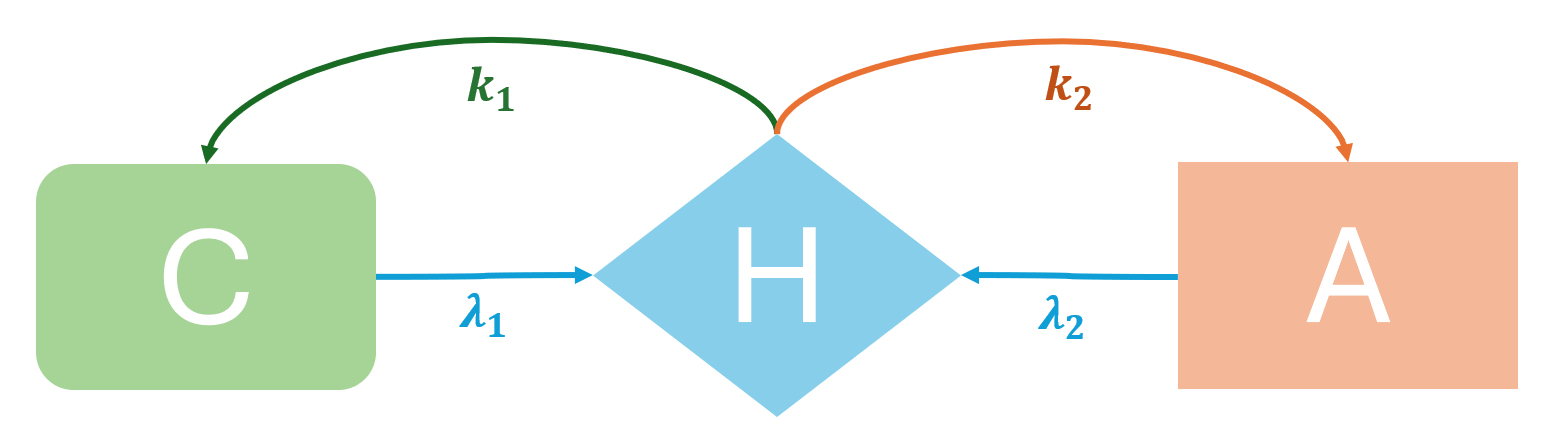
\includegraphics[width=0.72\linewidth]{1_corpo/figure/behavior_model_figure}
	\caption[Behavior model]{The figure represents the behavioral model developed, featuring three compartments: Heedless, Compliant, and Against, abbreviated as H, C, and A. The arrows indicate the inflows and outflows between these compartments.}
	\label{fig:behaviormodelfigure}
\end{figure}
The first mechanism is driven by peer pressure: the size of each group and the level of "persuasion" are the parameters that govern this process. It is mathematically modeled similarly to person-to-person disease transmission, as seen in the SIR-like mean-field model described in section \ref{subsubsec:p2p_transmission}. Instead, the return to the Heedless compartment is modeled as a "spontaneous decay" process: individuals naturally leave the Compliant and Against compartments and return to Heedless, transitioning spontaneously depending on the level of "fatigue" associated with maintaining the behavior.

To describe these transitions, different coefficients are introduced. The $k_1$ and $k_2$ are persuasion rates, while $\lambda_1$ and $\lambda_2$ represent fatigue rates. Their meanings are as follows: \begin{itemize} 
	\item $k_1$: persuasion rate from Heedless to Compliant; 
	\item $k_2$: persuasion rate from Heedless to Against; 
	\item $\lambda_1$: rate of leaving the Compliant behavior due to fatigue; 
	\item $\lambda_2$: rate of leaving the Against behavior due to fatigue. 
\end{itemize}

Finally, the resulting differential equations describing the model's dynamic are:
\begin{equation}
	\label{eq:behavioural_eq}
	\begin{cases}
		\dot{H} = -k_1 H C - k_2 H A + \lambda_1 C + \lambda_2 A \\
		\dot{C} = k_1 H C -  \lambda_1 C \\
		\dot{A} = k_2 H A -  \lambda_2 A\\
	\end{cases}
\end{equation}
Another assumption made to describe the model is the principle of mass conservation, meaning that the relationship $H + C + A = 1$ holds. Additionally, the initial conditions described in the previous section are translated as follows:
\begin{equation}
	\begin{cases}
		H(0) = 1 - C_0 - A_0\\
		C(0) = C_0 > 0\\
		A(0) = A_0 > 0\\
	\end{cases}
\end{equation}

\subsubsection{Behavior conversion number}

To simplify the understanding of the system's underlying dynamics, an analogy can be drawn with the reproduction number in epidemic models. By examining the system equations \ref{eq:behavioural_eq}, a relationship can be identified. From both the second and third equations, we can isolate the two coefficients (specifically $k_1 , \lambda_1 $, and  $k_2 , \lambda_2 $ and derive a new parameter, called "Behavior Conversion Rate", $\mathcal{B}$. This rate is the result of the ratio between the persuasion rate and the fatigue decay rate, and can be viewed as a measure of the transmission potential of social contagion. The general formula to calculate it is::
\begin{equation}
	\mathcal{B}_i =\frac{ k_i }{\lambda_i}  \qquad \text{with } i = 1, \text{or } 2.
	\label{eq:behave_rate}
\end{equation}
In the model presented here, $\mathcal{B}_1$ represents the Behavior Conversion Rate associated with the Compliant compartment, while $\mathcal{B}_2$, corresponds to the Against compartment. The results of different numerical simulations will now be displayed to demonstrate how the relationship between these two values influences the evolution of social contagion.

\subsection{Model simulation}
To represent different dynamics, four main cases are now presented. The coefficient values have been set appropriately to highlight different interesting situations in which the system can evolve. These cases represent the majority of possible scenarios:

\begin{itemize}
	\item[I] case: $\mathcal{B}_1, \mathcal{B}_2 <1$, $\mathcal{B}_1 >  \mathcal{B}_2$, and $\lambda_1 > \lambda_2$.
	\item[II] case: $\mathcal{B}_1, \mathcal{B}_2 >1$, $\mathcal{B}_1 =  \mathcal{B}_2$, and $\lambda_1 < \lambda_2$.
	\item[III] case: $\mathcal{B}_1, \mathcal{B}_2 >1$, $\mathcal{B}_1 >  \mathcal{B}_2$, and $\lambda_1 = \lambda_2$.
	\item[IV] case: $\mathcal{B}_1, \mathcal{B}_2 >1$ and $\mathcal{B}_1 >  \mathcal{B}_2$, and $\lambda_1 < \lambda_2$.
\end{itemize}

The values $k_1$, and $k_2$ are calculated from the formula of $\mathcal{B}_1$, and $\mathcal{B}_2$.

In Figure \ref{fig:model__behavior_sim_1}, it is evident that when both Behavior conversion numbers are less than one, social contagion does not spread: even though, in this case, the Compliant and Against compartments together represent $60\%$ of the total population at the beginning of the simulation, they clearly tend to zero over time. In contrast, the right panel shows the case where the two $\mathcal{B}$ values are equal and greater than one. To emphasize the importance of the fatigue rate, it is shown that with a lower $\lambda_2$ value than $\lambda_1$, the Against compartment becomes dominant by the end of the simulation. 
\begin{figure}[h]
	\centering
	\subfloat[][\emph{$\mathcal{B}_1, \mathcal{B}_2 <1$, $\mathcal{B}_1 >  \mathcal{B}_2$, and $\lambda_1 > \lambda_2$.}]
	{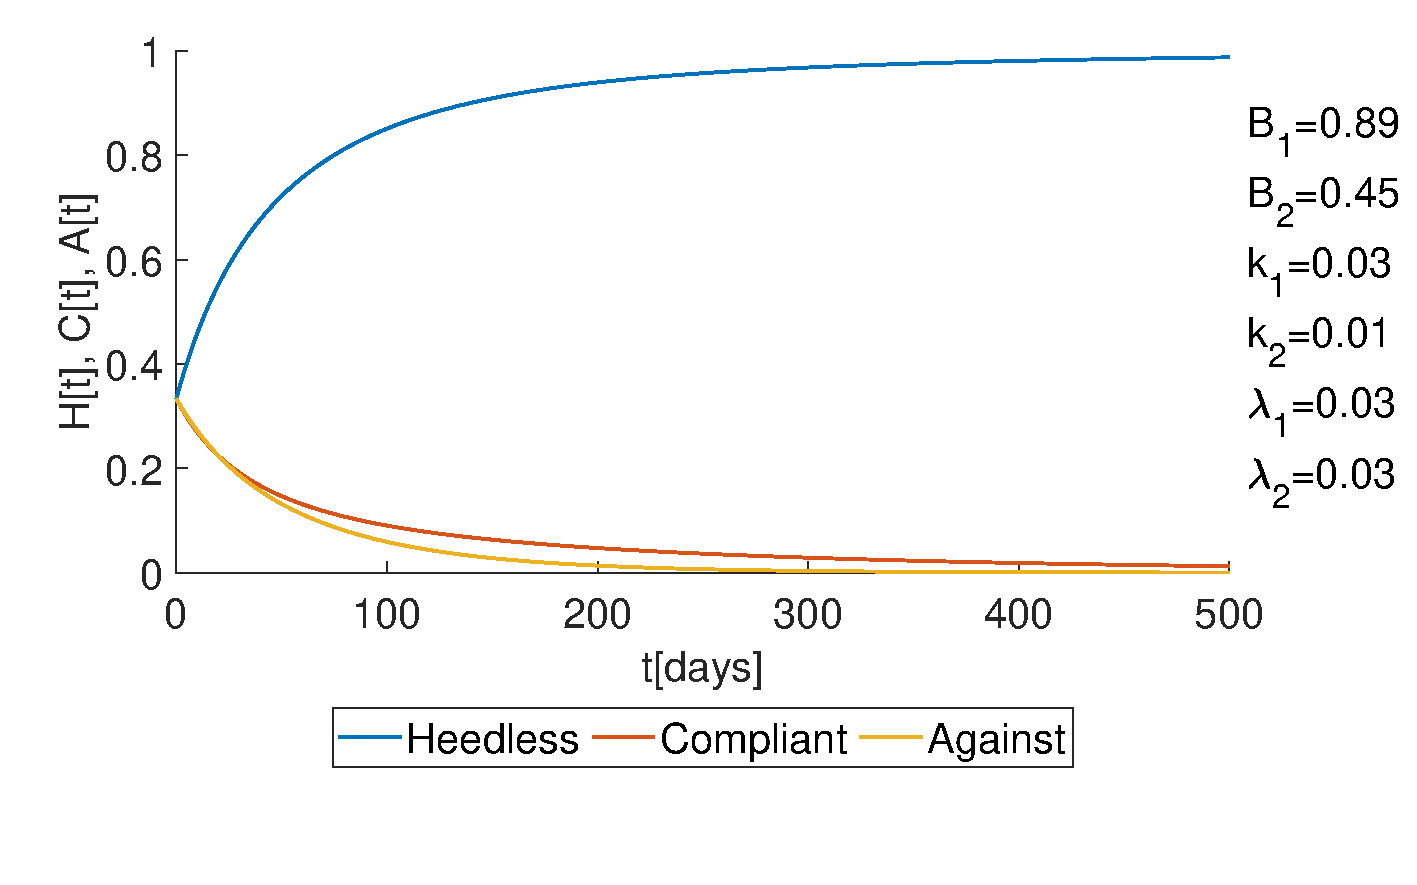
\includegraphics[width=0.48\linewidth]{1_corpo/figure/behavioural_equilibrium/behavior_B1_B2_less_1}} \quad
	\subfloat[][\emph{$\mathcal{B}_1, \mathcal{B}_2 >1$, $\mathcal{B}_1 =  \mathcal{B}_2$, and $\lambda_1 < \lambda_2$.}]
	{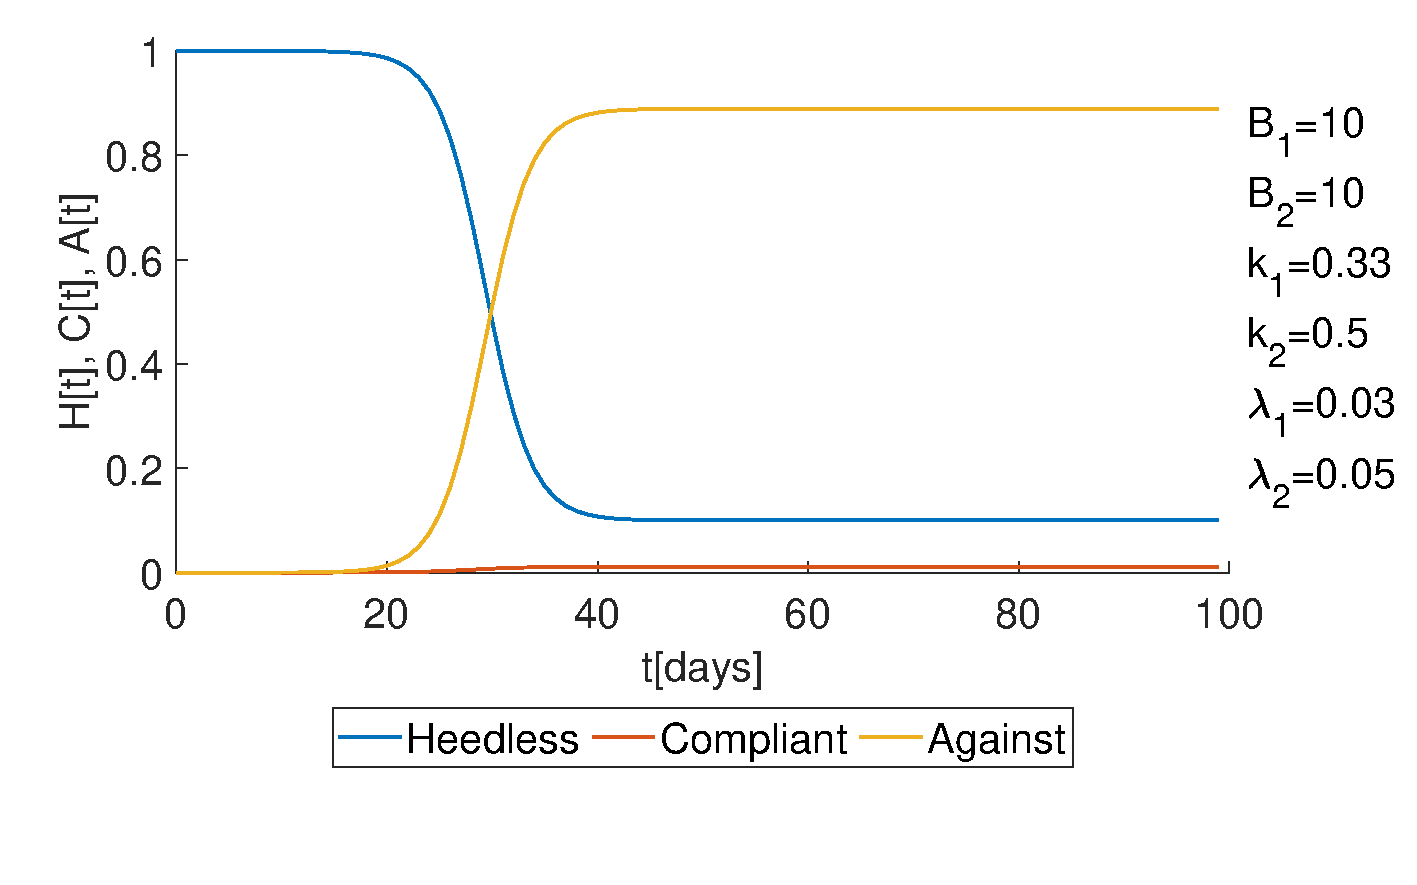
\includegraphics[width=0.48\linewidth]{1_corpo/figure/behavioural_equilibrium/behavior_B1_equal_B2}} \\
	\caption[Behavioural model simulation first]{Behavioural system dynamics first two cases.}
	\label{fig:model__behavior_sim_1}
\end{figure}

Figure \ref{fig:model__behavior_sim_2} illustrates two other interesting scenarios. On the left, we observe the dynamics when one of the $\mathcal{B}$ values is greater than the other, and both $\lambda$ values are the same. It is straightforward to understand that this dynamic would also occur if, with the same values, the $\lambda$ of the dominant behavior were greater than the other, as a larger $\lambda$ would result in a higher $k$ (persuasion rate). The right panel, however, presents a particularly intriguing situation. Here, a lower $\lambda_1$ compared to $\lambda_2$, combined with $k_2 > k_1$, leads to an initial rapid spread of the Against group, even though $\mathcal{B}_2 < \mathcal{B}_1$! It is only after some time that the system evolves to the final equilibrium, which matches the left scenario's result, as the $\mathcal{B}$ values are the same in both simulations.

\begin{figure}[h]
	\centering
	\subfloat[][\emph{$\mathcal{B}_1, \mathcal{B}_2 >1$, $\mathcal{B}_1 >  \mathcal{B}_2$, and $\lambda_1 = \lambda_2$.}]
	{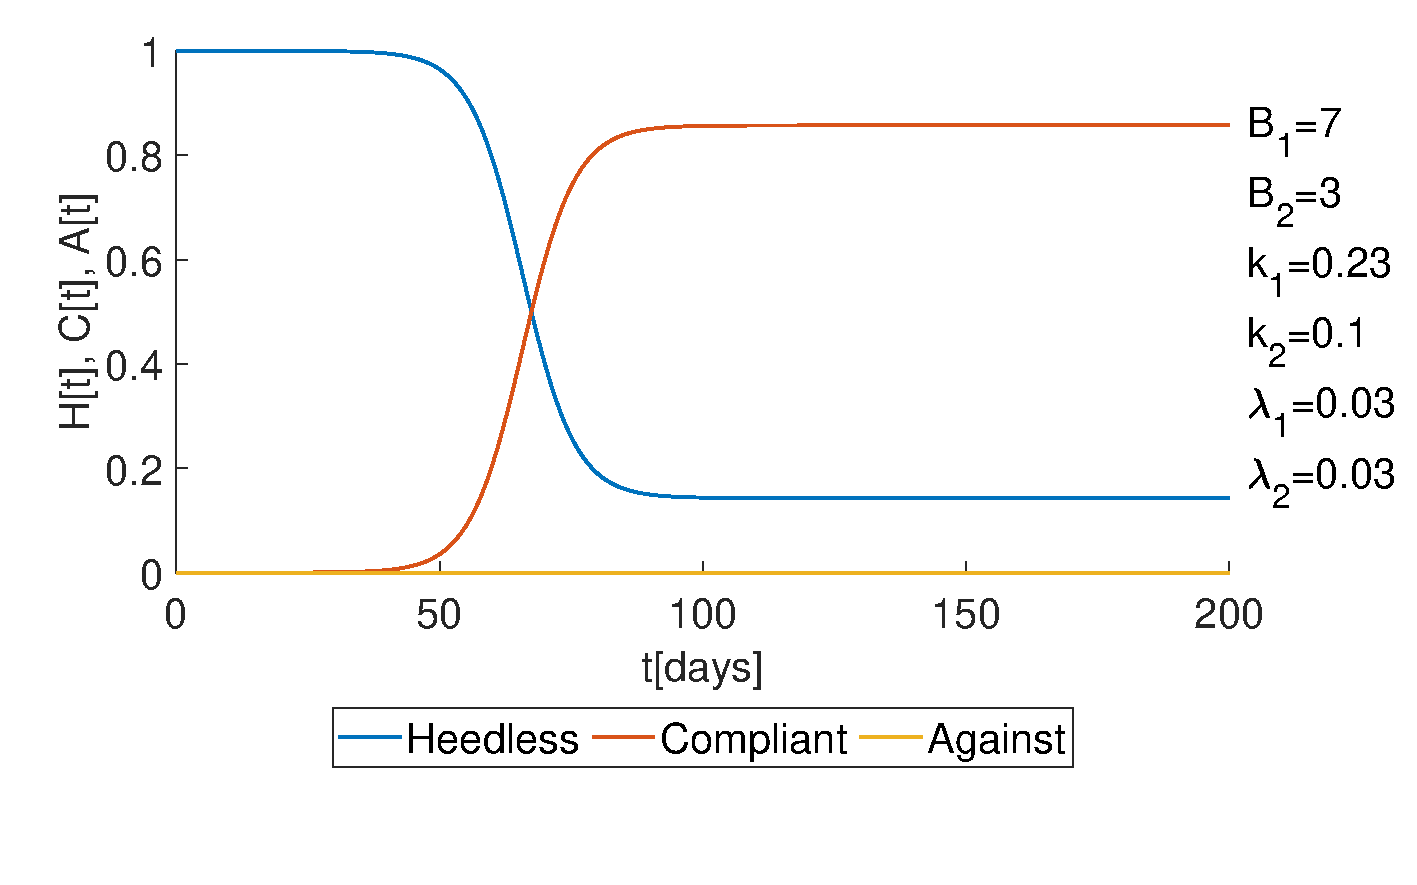
\includegraphics[width=0.48\linewidth]{1_corpo/figure/behavioural_equilibrium/behavior_B1_mag_B2_k1_mag_k2}} \quad
	\subfloat[][\emph{$\mathcal{B}_1, \mathcal{B}_2 >1$ and $\mathcal{B}_1 >  \mathcal{B}_2$, and $\lambda_1 < \lambda_2$.}]
	{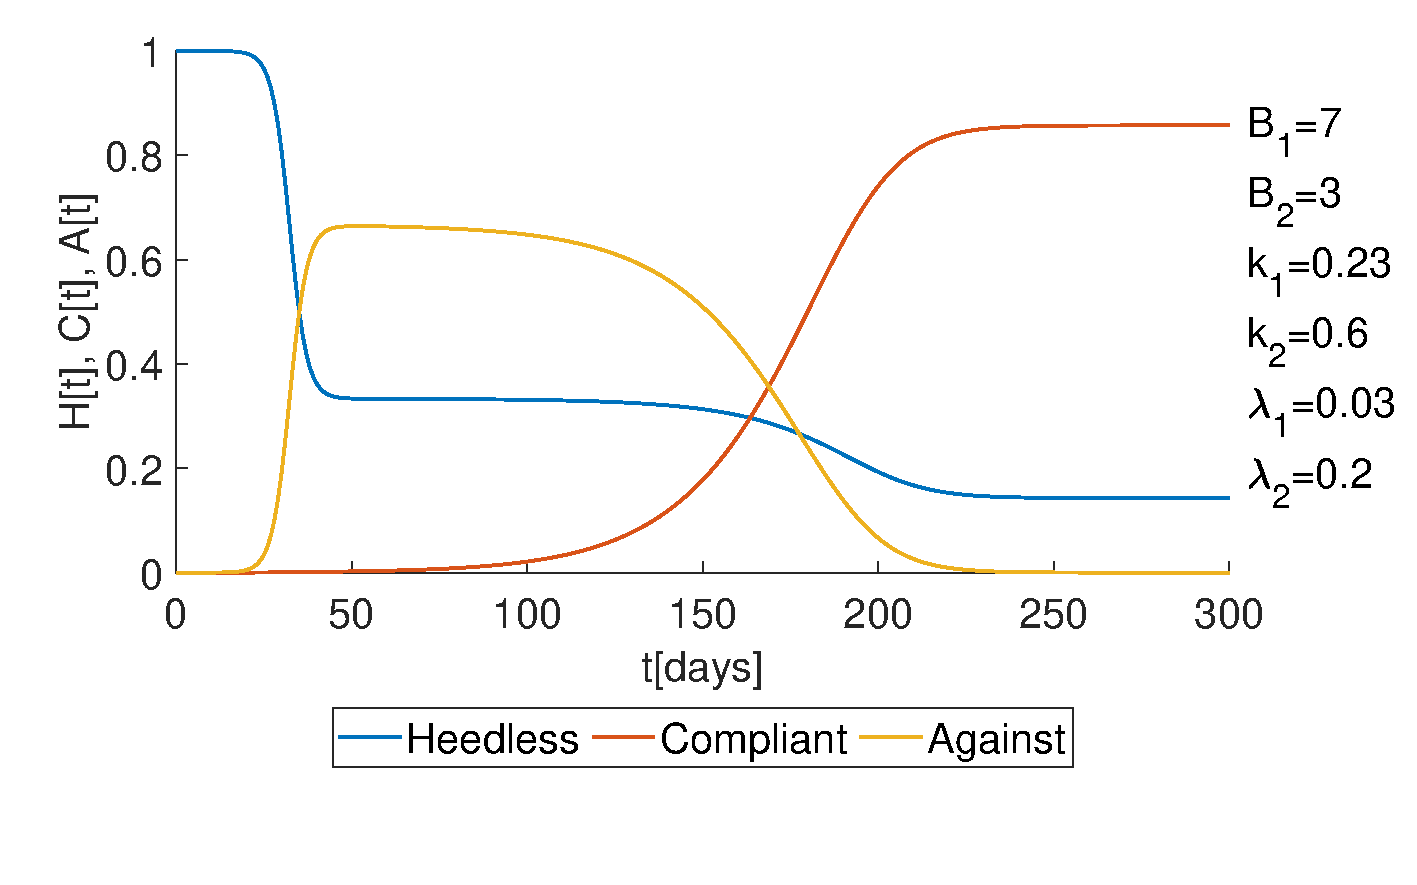
\includegraphics[width=0.48\linewidth]{1_corpo/figure/behavioural_equilibrium/behavior_B1_mag_B2_k2_mag_k1}} \\
		\caption[Behavioural model simulation second]{Behavioural system dynamics second two cases.}
	\label{fig:model__behavior_sim_2}
\end{figure}

\subsubsection{Equilibrium and stability analysis}
To enhance understanding of the system, for the four cases presented before an analysis is performed, and, where present, the stability of their equilibria was determined.

As observed, the system’s final equilibrium values vary according to parameter values. Specifically, the coefficients were combined to produce two Behavior conversion numbers, $\mathcal{B}_1$ and $\mathcal{B}_2$.

One way to identify and visualize the system’s equilibrium for a specific parameter set is through nullclines. These were calculated for each case, and the results are presented here. To better visualize nullclines in a two-dimensional graph, the system can be reduced from three to two equations using the mass conservation assumption, yielding the following relationship: $1=H+C+A$ The first two equations are then rewritten, substituting the $A$ term, resulting in a two-equation system with two unknowns. By calculating the nullclines and varying the values of $\mathcal{B}_1$ and $\mathcal{B}_2$, we examine different scenarios. This reduction from the original system of three equations \ref{eq:behavioural_eq}  results in the following two-equation system: 
\[
\begin{cases}
	\dot{H} = -k_1 H C - k_2 (1-H-C) H + \lambda_1 C + \lambda_2 (1-H-C)\\
	\dot{C} = k_1 H C - \lambda_1 C
\end{cases}
\]
To simplify the readability and use a notation more familiar for plotting, the $H, C$ symbols have been substituted with respectively $x, y$. So equations become:
\begin{equation}
\label{eq:system_nullclines}
\begin{cases}
	\dot{x} = -k_1 y x - k_2 (1-y-x) x + \lambda_1 y + \lambda_2 (1-y-x)\\
	\dot{y} = k_1 y x - \lambda_1 y
\end{cases}
\end{equation}
The nullclines lines can be calculated imposing $\dot{x} = 0$ and $\dot{y} = 0$. Solving the system with this condition applied gives the following two equations. For the first nullcline, with $\dot{x} = 0$:

\begin{equation}
 y = \frac{x(k_2 - k_2 x + \lambda_2)  \lambda_2}{x(k_2 - k_1)+ \lambda_1- \lambda_2}
\end{equation}
and for the second with $\dot{y} = 0$
\[x = \frac{\lambda_i}{k_i} = 1/\mathcal{B}_i \qquad \text{with } i = 1, \text{or } 2.
\]
The selection of the correct $\mathcal{B}_i$ to use for the second nullcline depends on
the comparison between the two reproductive ratio values. Seeing the result of the simulation, it is understood that the larger value should be chosen, as it represents the behavior that will dominate at equilibrium, while the other behavior will tend toward zero. Only in the case where the the $\mathcal{B}_1, \mathcal{B}_2 < 1$ these rule not holds, because the result of the secon nullcline found with the formula is out of the domain of existence (i.e $x > 1$, while the Compliant, $x$ are a value comprised between $[0,1]$.)
The first nullcline existence condition can be calculated, imposing that the denominator must be not equal to zero. The result is
\[ x \neq \frac{\lambda_2-\lambda_1}{k_2 - k_1} \]
These value of $x$ is in the interval $[0,1]$ only if $\lambda_2>\lambda_1$ and $k_2 > k_1$, or $\lambda_2<\lambda_1$ and $k_2 < k_1$. The second nullcline instead, exist always iff $k_i \neq 0$.


Now the four primary cases of the system’s evolution, with stability analyses conducted for the identified equilibria are presented.
%%%%%%%%%%%%%%%%%%

\textbf{I case: }$\mathcal{B}_1, \mathcal{B}_2 <1$, $\mathcal{B}_1 >  \mathcal{B}_2$, and $\lambda_1 > \lambda_2$. \\
If both the "reproduction rates" have a value lower than one, the stable equilibrium is the one in which both Compliant and Against goes to zero. 

From the nullcline plot, visible in the left figure \ref{fig:r1r2less1dyn}, it can be seen that there is not an intersection. The plot of the second nullcline result in a vertical line with a value grater than one. In this condition the only equilibrium is the one for which $H = 1$ and both $A$ and $C$ are equal to zero. 

With the Routh-Hurwitz criteria the stability of this point is verified. To evaluate if the criteria is satisfied the Jacobian matrix of the system is calculated. Then the equilibrium is used to evaluate the trace and determinant of the system in this value. To see if the equilibrium satisfies Routh-Hurwitz condition it must holds:
\begin{itemize}
	\item trace(J) $< 0$
	\item det(J) $> 0$
\end{itemize}
 
The Jacobian of the system of equation \ref{eq:system_nullclines} is
\begin{equation}
J = \begin{bmatrix}
	-k_1 y -k_2 +k_2 y+2 k_2 x- \lambda_2 & -k_1 x + k_2 x + \lambda_1-\lambda_2 \\
	k_1 y & k_1 x - \lambda_1
\end{bmatrix}
\end{equation}
The trace of $J$ is
\begin{equation}
	trJ = -k_1 y -k_2 +k_2y + 2 k_2 x - \lambda_2 -\lambda_1 +k_1 x
\end{equation}
Its determinant is instead
\begin{equation}
	detJ = k_2 \lambda_1 + \lambda_1 \lambda_2 + 2 k_1 k_2 x^2 - k_1 k_2 x - k_1 \lambda_2 x - 2\cdot k_2 \lambda_1 x + k_1 \lambda_2 y - k_2 \lambda_1 y
\end{equation}
In this case the equilibrium point is all population Heedles, so $x = 1$, and $y = 0$. Calculating in this point the trace and determinant of the Jacobian, it is found $trJ(1,0) =-209/12000$, and $detJ = 121/2400000$. So, the equilibrium is locally asymptotically stable, because satisfies Routh-Hurwitz condition. 
\begin{figure}[h]
	\centering
	\subfloat[][\emph{$\mathcal{B}_1, \mathcal{B}_2 <1$, $\mathcal{B}_1 >  \mathcal{B}_2$, and $\lambda_1 > \lambda_2$.}]
	{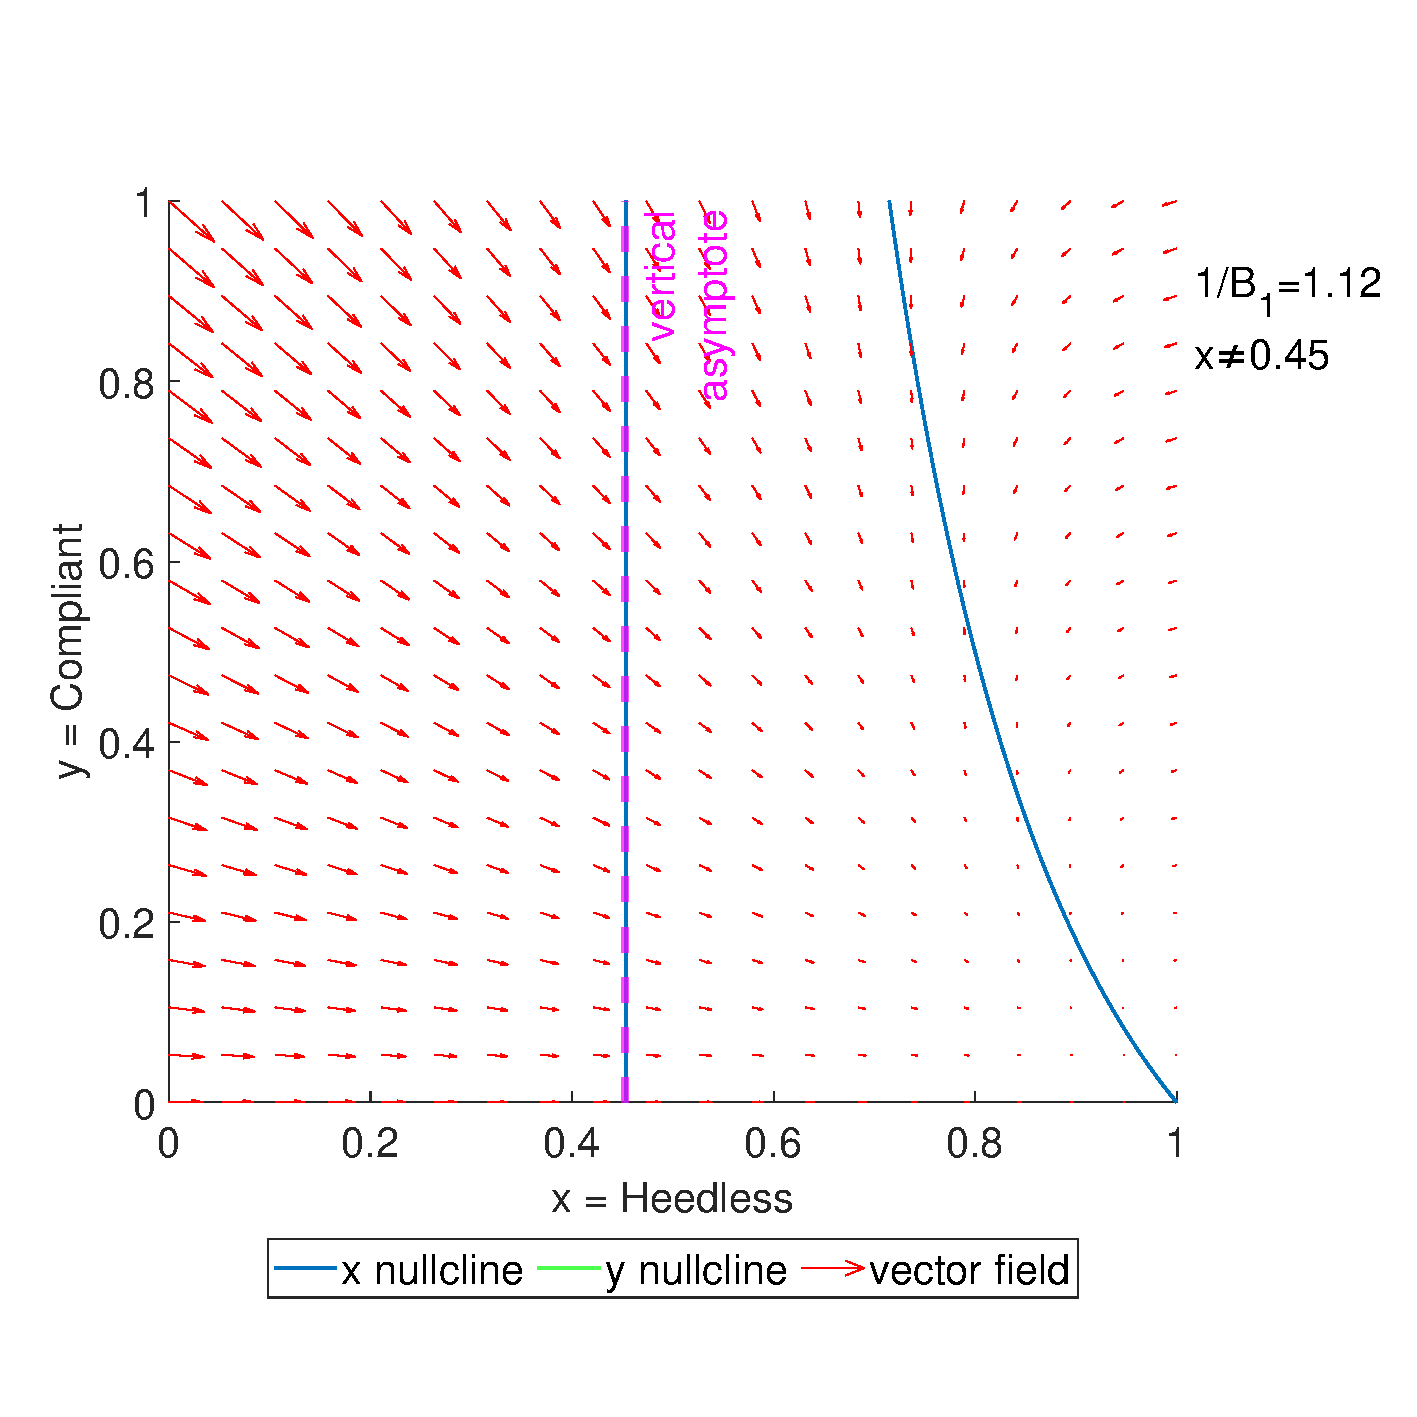
\includegraphics[width=0.48\linewidth]{1_corpo/figure/behavioural_equilibrium/Pr_nullcline_B1_B2_less_1}} \quad
	\subfloat[][\emph{$\mathcal{B}_1, \mathcal{B}_2 >1$, $\mathcal{B}_1 =  \mathcal{B}_2$, and $\lambda_1 < \lambda_2$}]
	{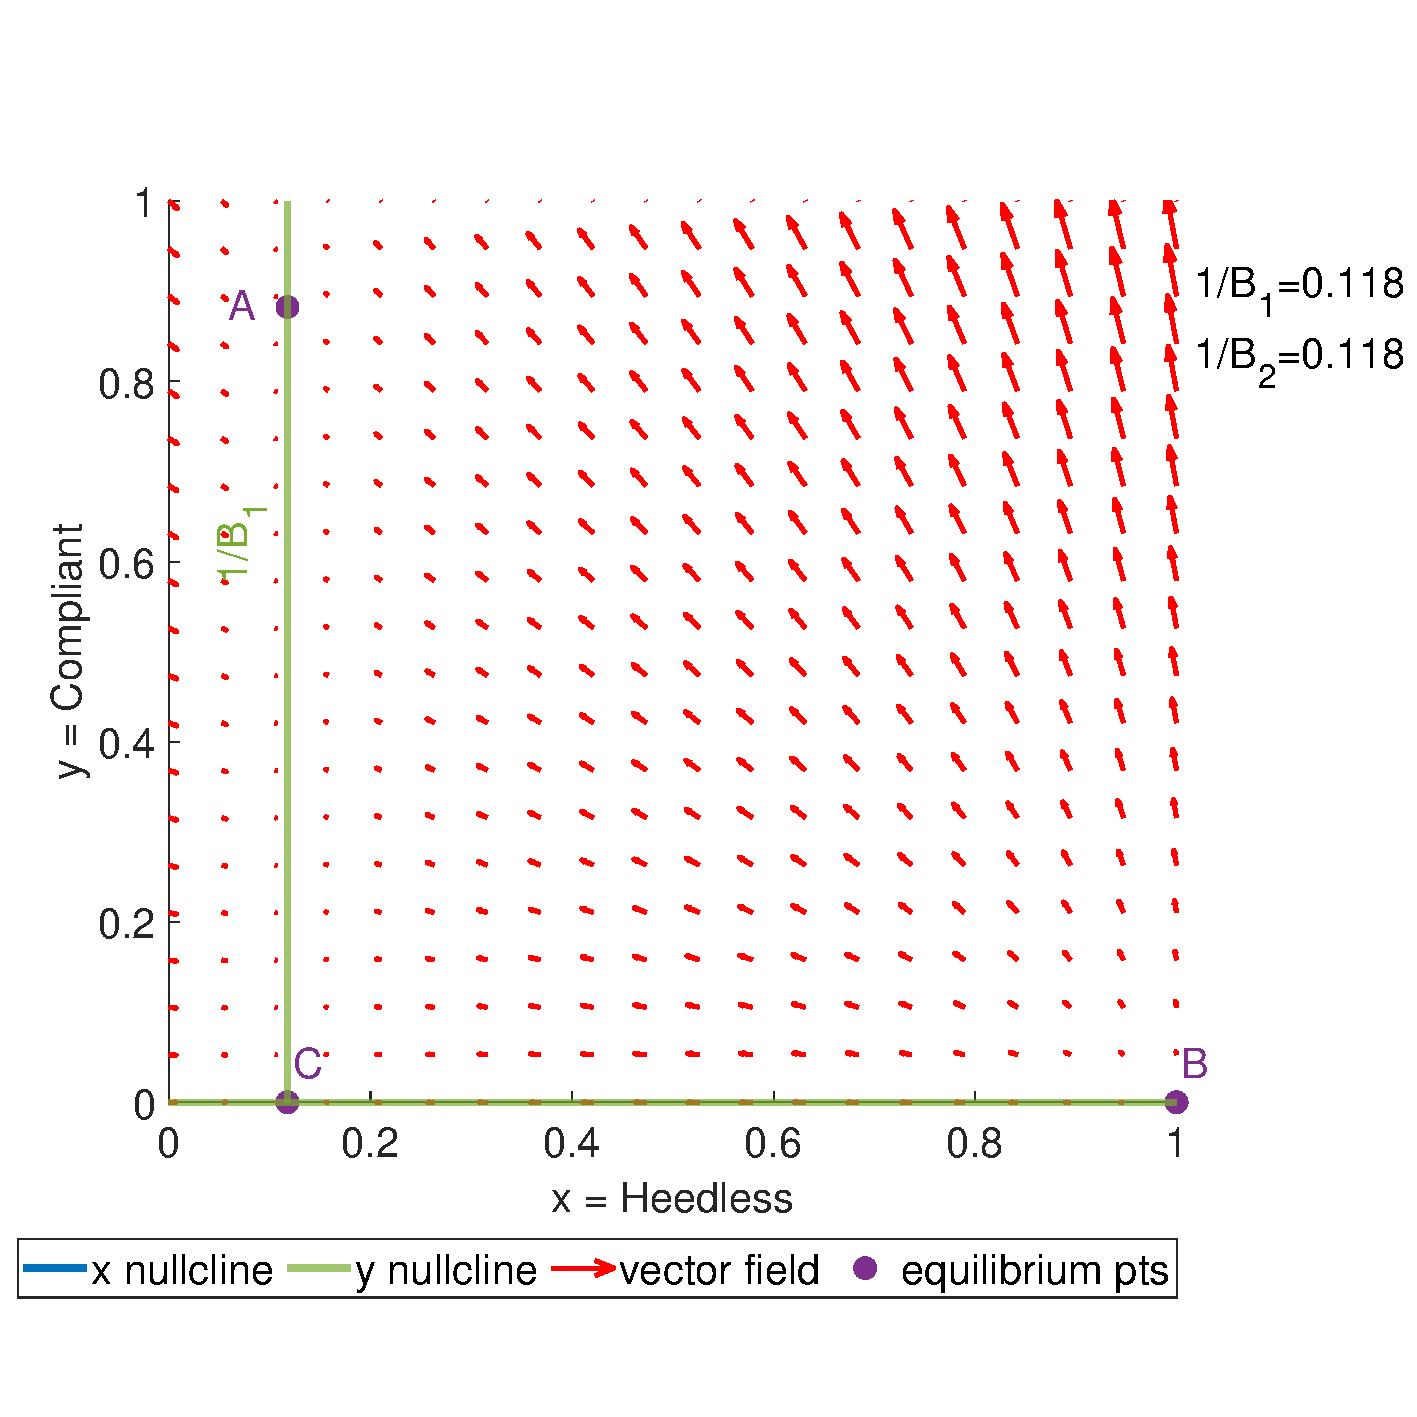
\includegraphics[width=0.48\linewidth]{1_corpo/figure/behavioural_equilibrium/Pr_nullcline_B1_B2_equal}} \\
	\caption[Nullclines first figure]{Nullclines plots of the first two situations analyzed.}
	\label{fig:r1r2less1dyn}
\end{figure}
%%%%%%%%%%%%%%%%%%

\textbf{II case: } $\mathcal{B}_1, \mathcal{B}_2 >1$, $\mathcal{B}_1 =  \mathcal{B}_2$, and $\lambda_1 < \lambda_2$.\\
This second situation is the most difficult to analyse. In fact, due to the equal value of the two influence processes, the final equilibrium of the compartments cannot be calculated using only the previous relations, but depends also on the initial condition. 
The Heedless compartment can be calculated using the same equation of previous cases, and the same value is found using both $x = \lambda_1/k_1$ and $x = \lambda_2/k_2$. So the final value of $x$ at equilibrium here is $\bar{x} = 0.12$. As it can be seen from the system evolution \ref{fig:model__behavior_sim_1},and nullcline plots \ref{fig:r1r2less1dyn}  ,at the equilibrium the Against and Compliant groups are formed by a subdivision of the $1 - \bar{x}$ part. The initial condition have an influence on how this subdivision is composed. Using the Routh-Hurwitz criterium nothing can be said on this equilibrium because the determinant of the Jacobian have a null value.
%%%%%%%%%%%%%%%%%%%%%%%%%%%%

\textbf{III case:} $\mathcal{B}_1, \mathcal{B}_2 >1$, $\mathcal{B}_1 >  \mathcal{B}_2$, and $\lambda_1 = \lambda_2$. \\
In this scenario, as visible in figure \ref{fig:nullcline_B1_mag_B2}, the Against compartment tend to zero, so the equilibrium point can be calculated as $\bar{x} = \lambda_1/k_1$ and $\bar{y} = 1 - \lambda_1/k_1 $. 
The nullcline resulting plot is visible in \ref{fig:nullcline_B1_mag_B2}. 

The equilibrium found as intersection of the two lines correspond to the one calculated with the numerical equation. 
Both condition holds: $trJ(\bar{x},\bar{y}) = -23/105$, and $detJ(\bar{x},\bar{y}) = 2/525$, so the solution is locally asymptotically stable and does not depends on the initial condition.
%%%%%%%%%%%%%%%%%%%%%%%%%%%%
\textbf{III bis case: }$\mathcal{B}_1, \mathcal{B}_2 >1$, $\mathcal{B}_1 <  \mathcal{B}_2$, and $\lambda_1 = \lambda_2$.
The evolution of the system has an opposite behaviour w.r.t the previous case. So here, is the Compliant compartment that tend to zero at equilibrium. 

The equilibrium point can be calculated as $\bar{x}= \lambda_2/k_2$ and $\bar{z} = 1 - \lambda_2/k_2$. 
Also this equilibrium is locally asymptotically stable. 
\begin{figure}[h]
	\centering
	\subfloat[][\emph{ $\mathcal{B}_1, \mathcal{B}_2 >1$, $\mathcal{B}_1 >  \mathcal{B}_2$, and $\lambda_1 = \lambda_2$.}]
	{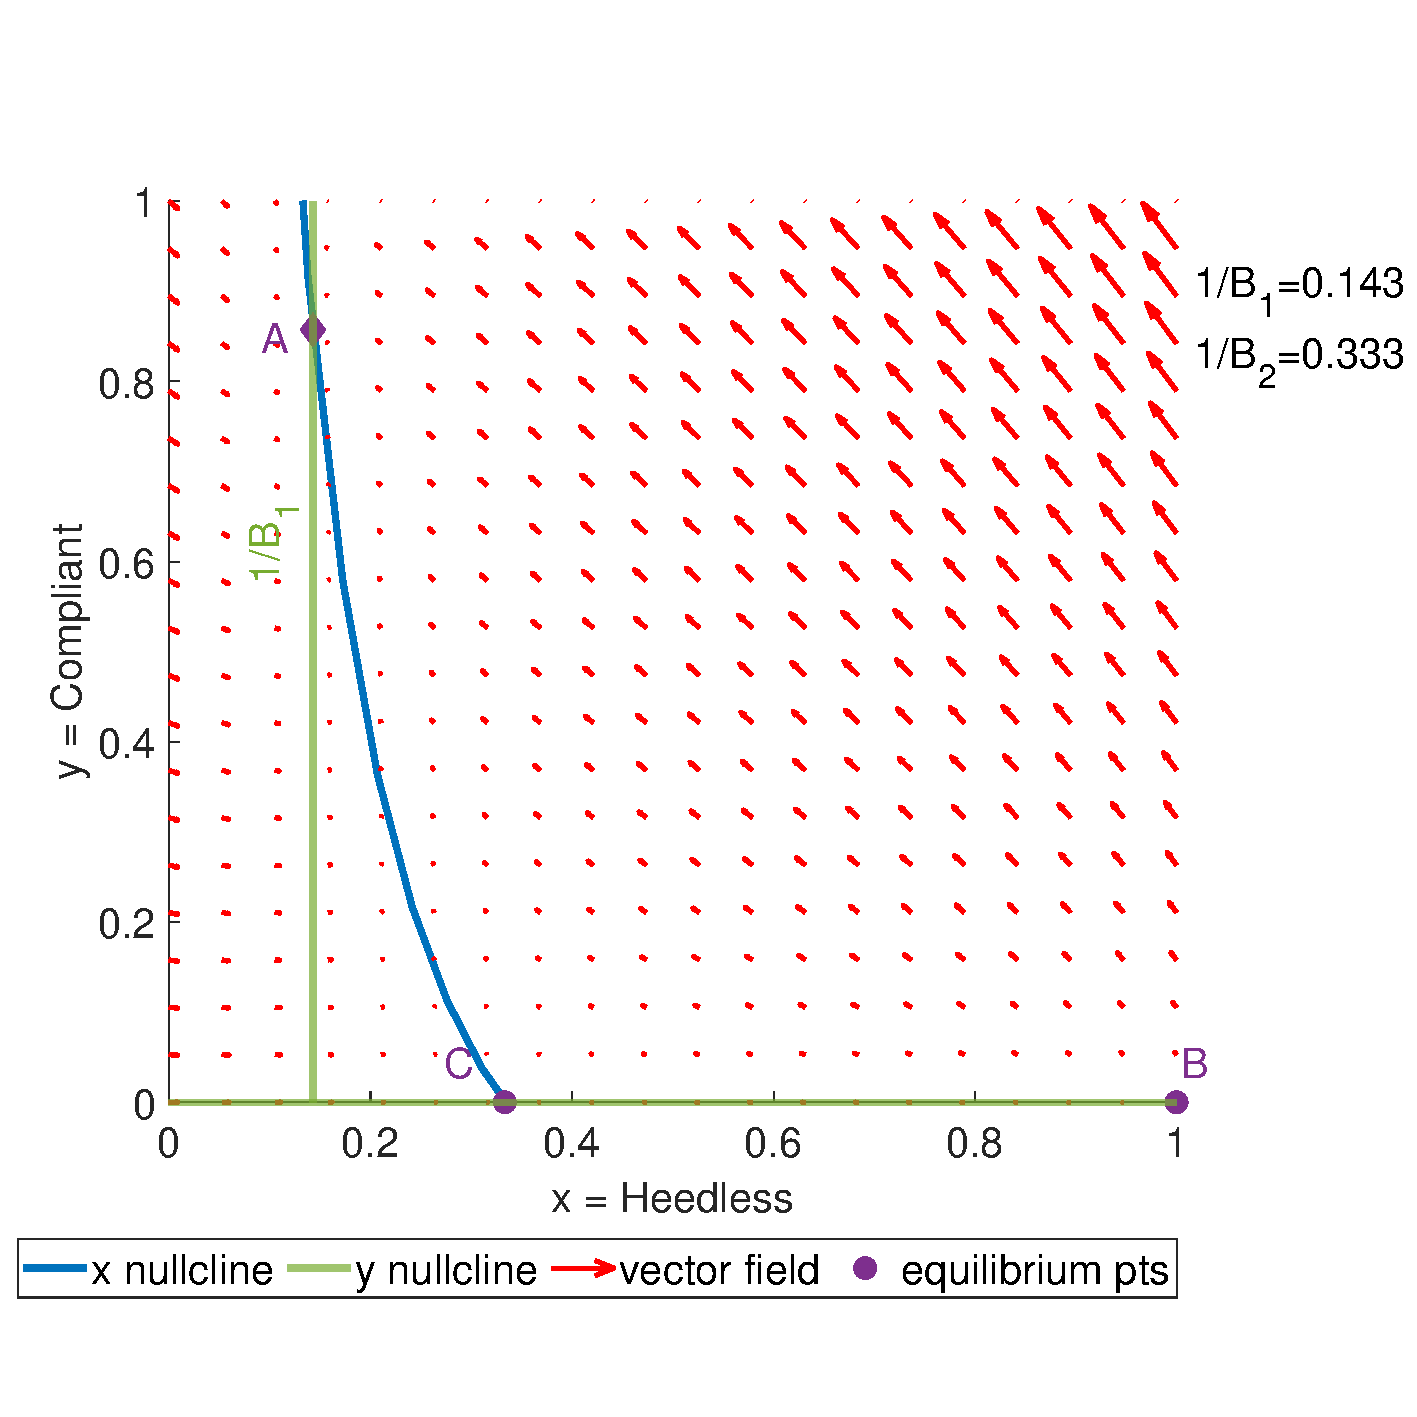
\includegraphics[width=0.48\linewidth]{1_corpo/figure/behavioural_equilibrium/Pr_nullcline_B1_mag_B2}} \quad
	\subfloat[][\emph{ $\mathcal{B}_1, \mathcal{B}_2 >1$ and $\mathcal{B}_1 >  \mathcal{B}_2$, and $\lambda_1 < \lambda_2$.}]
	{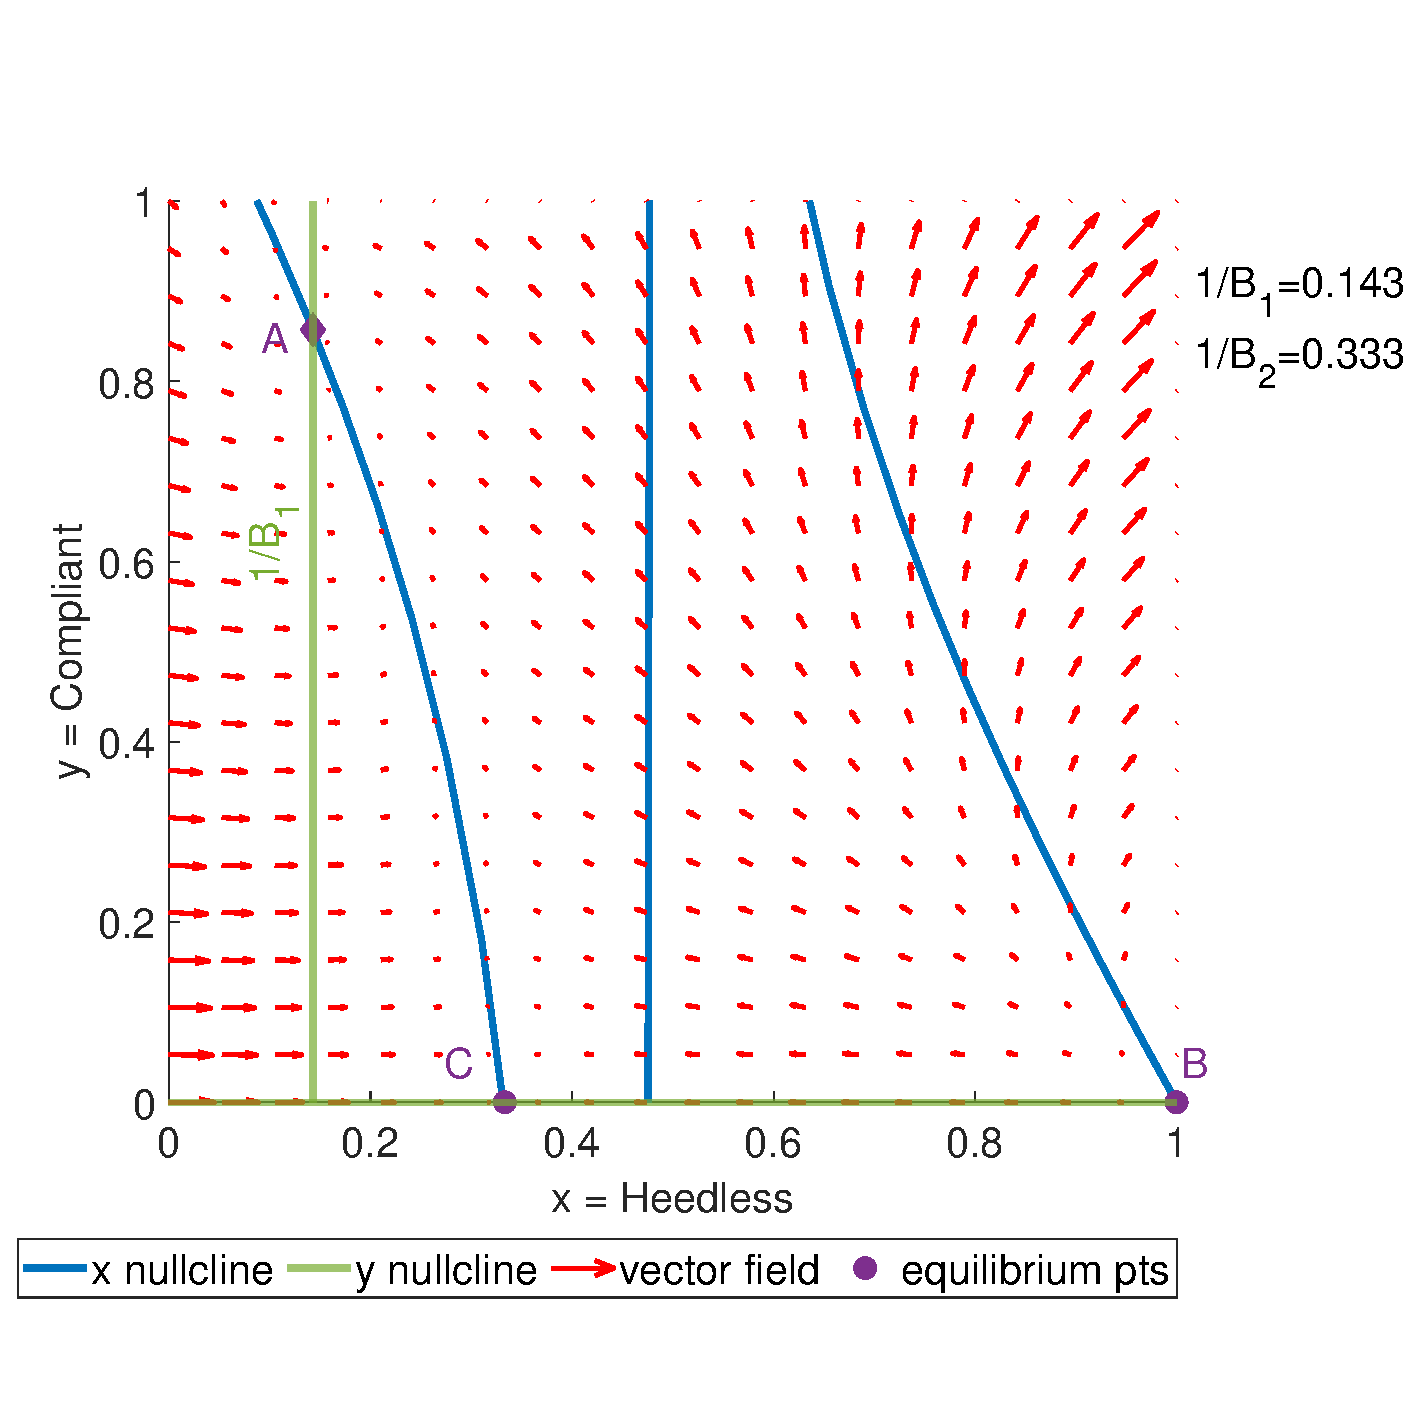
\includegraphics[width=0.48\linewidth]{1_corpo/figure/behavioural_equilibrium/Pr_nullcline_B1_mag_B2_lambda2_mag}} \\
	\caption[Nullclines second figure]{Nullclines plots of the second two situations analyzed.}
	\label{fig:nullcline_B1_mag_B2}
\end{figure}

\textbf{IV case: } $\mathcal{B}_1, \mathcal{B}_2 >1$ and $\mathcal{B}_1 >  \mathcal{B}_2$, and $\lambda_1 < \lambda_2$. \\
In this situation, the equilibrium has the same value, of the III case, and also the stability condition are verified. However, the nullcline plot is very different. The vertical asymptote is clearly visible in the middle of the left panel in figure \ref{fig:nullcline_B1_mag_B2}. Also the vector field in the two cases are different, and as show in figure \ref{fig:model__behavior_sim_2}, the system initially evolve to a first equilibrium, corresponding to $\bar{x} = \lambda_2/k_2$, $y = 0$, and $\bar{z} = 1 - \lambda_2/k_2$, but this equilibrium not satisfies Routh-Hurwitz: calculating the value, it is in fact found $trJ > 0$, and $detJ= 0$.


\subsubsection{Behavioural model experiment}
To better comprehend all the possible scenarios that can emerge with the behavioural model a simulation is performed. Four vectors are defined, one for each parameter of the model. A different simulation for each combination of the coefficient is then roll out. In this case the value of the parameters is kept constant during each simulation.
The range of variation of each parameter is the following:
\begin{itemize}
	\item $B_1$ between $0.1$ and $10$
	\item $B_2$ between $0.1$ and $10$
	\item $\lambda_1$ between $1/2$ and $1/40$ $d^{-1}$
	\item $k_1$ between $1/2$ and $1/40$ $d^{-1}$
\end{itemize}
It have been chosen these ranges because it is ipothesized that for the "fatigue" rate, a range between two and forty days can be realistic, this range has also been used in \cite{trova e cita world in data}. For the behavior conversion rate instead are chosen values that comprehend both a low and a high number of transition rates.  
We observe the evolution of the dynamics of all the states, and to present a summary of the effects we collect for each simulation data such as the final value of the compartment, the max peak value and the corresponding time in which the peak occur. 
Also here, for the sensitivity plots realization, the reproduction rates deriving from the combination of coefficients, equation \eqref{eq:behave_rate}, are used. 

The first plots \ref{fig:subfig_sensitivity_behavioural} are heat maps about the final value reached by various compartments, varying $B_1$ and $B_2$.

\begin{figure}[h]
	\centering
	\subfloat[][\emph{Final Compliant compartment}]
	{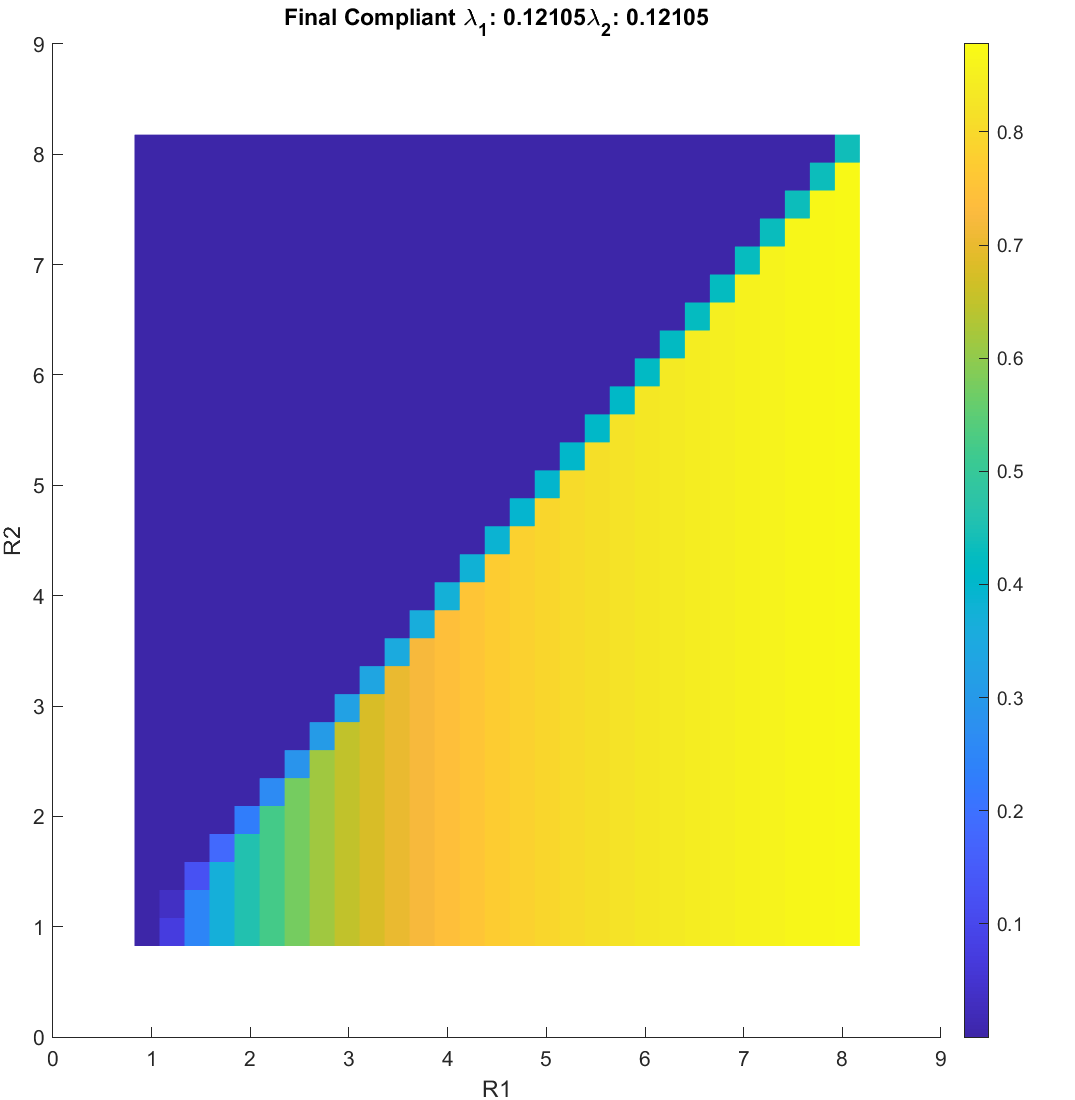
\includegraphics[width=.47\textwidth]{1_corpo/figure/behavioural_equilibrium/final_compliant_sensitivity}} \quad
	\subfloat[][\emph{Final Against compartment}]
	{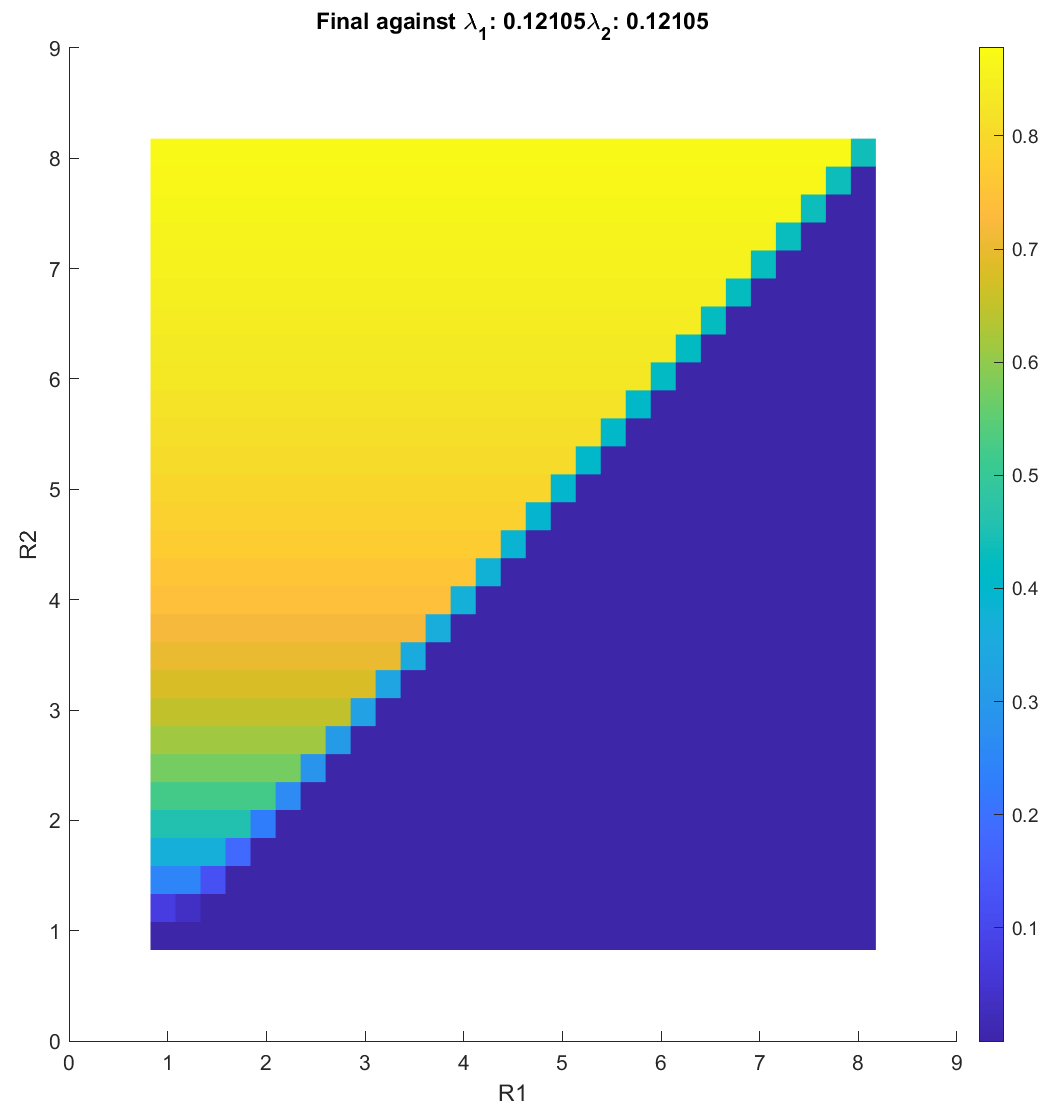
\includegraphics[width=.47\textwidth]{1_corpo/figure/behavioural_equilibrium/final_against_sensitivity}} \\
	\subfloat[][\emph{Final Careless compartment}]
	{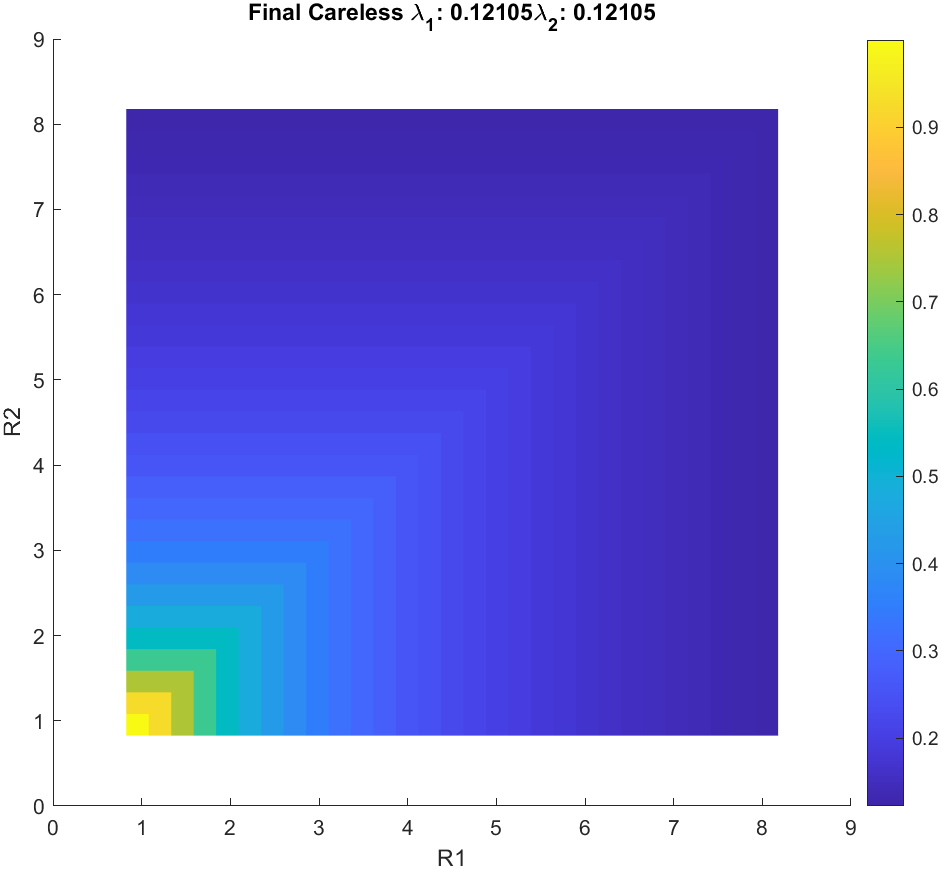
\includegraphics[width=.47\textwidth]{1_corpo/figure/behavioural_equilibrium/final_careless_sensitivity}}
	\caption[Final Behavioural compartments]{The final value reached at equilibrium by every compartment in the behavioural model.}
	\label{fig:subfig_sensitivity_behavioural}
\end{figure}

In these pictures is clearly visible the threshold effect observed in the stability analysis performed earlier. While one of the reproduction ratios becomes larger than the other, the system equilibrium is composed by the dominant group and a portion of Careless individuals.The greater is the ratio, the  smaller is the size at equilibrium of the Careless. 

Another figure in which this threshold effect can be observed is \ref{fig:subfig_sensitivity_behavioural_r1}.

\begin{figure}[h]
	\centering
	\subfloat[][\emph{Final Compliant compartment}]
	{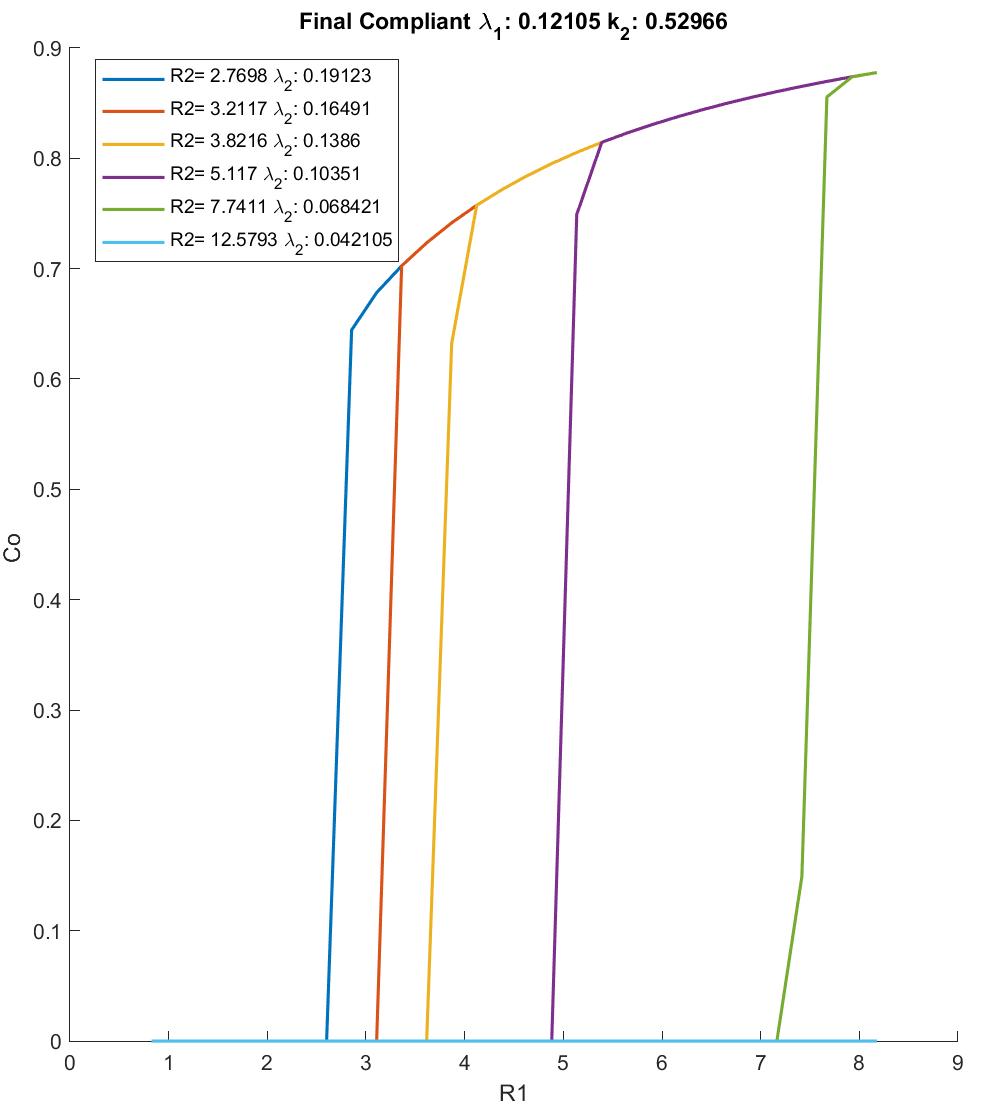
\includegraphics[height=.45\textwidth]{1_corpo/figure/behavioural_equilibrium/final_compliant_r1}} \quad
	\subfloat[][\emph{Final Against compartment}]
	{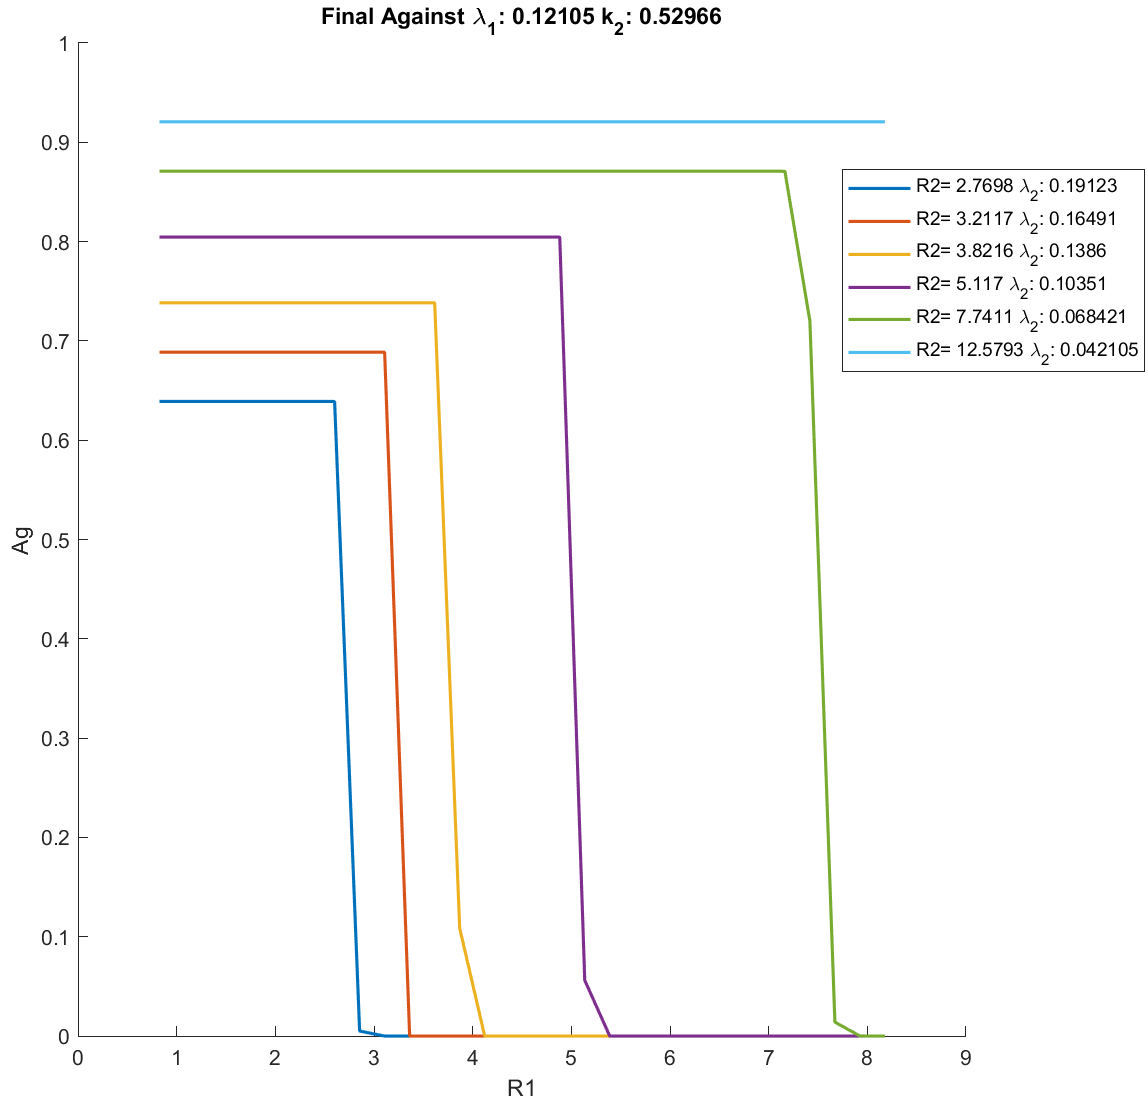
\includegraphics[height=.45\textwidth]{1_corpo/figure/behavioural_equilibrium/final_against_r1}} \\
	\subfloat[][\emph{Final Careless compartment}]
	{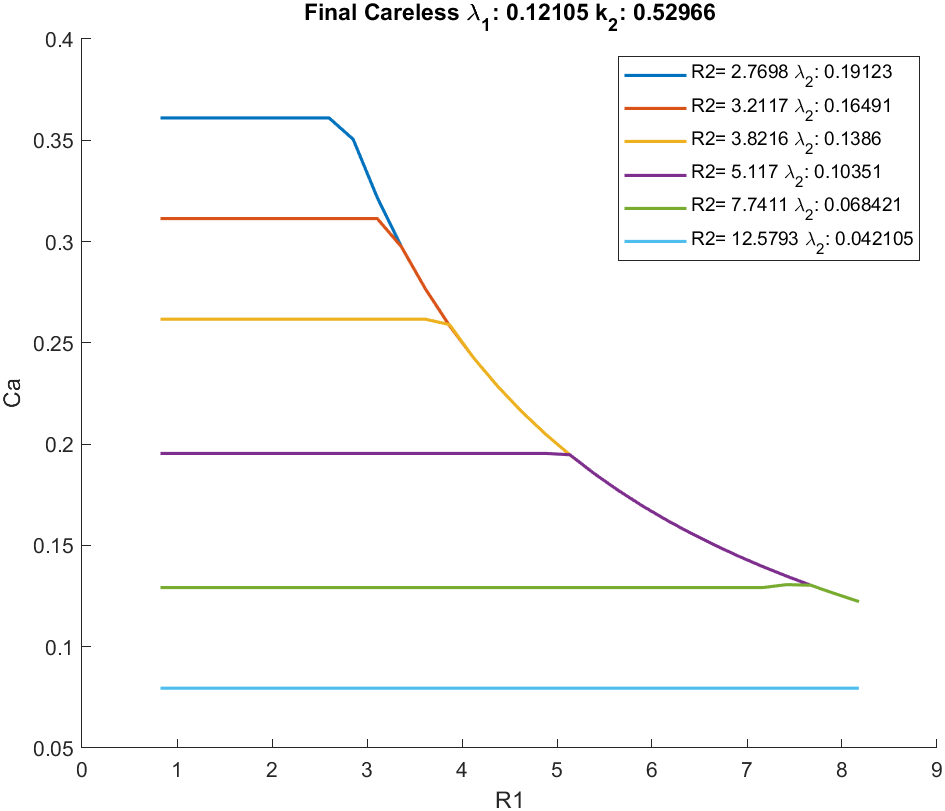
\includegraphics[height=.45\textwidth]{1_corpo/figure/behavioural_equilibrium/final_careless_r1}}
	\caption[Final Behavioural compartments varying $R_1$]{The final value reached at equilibrium by every compartment in the behavioural model varying the $R_1$ coefficient w.r.t different $R_2$ values.}
	\label{fig:subfig_sensitivity_behavioural_r1}
\end{figure}
The plots show how, for a fixed values of $\lambda_1$ and $k_2$, change the size at equilibrium of the system, varying the $k_1$ coefficient. To highlight the threshold effect due to the comparison of reproduction rates, on the x-axis is plotted the $R_1$  coefficient, that can be calculated knowing the value of  $\lambda_1$ and $k_1$. For the same reason, different $R_2$ situations are represented. 

The threshold effect is clearly visible also here. Looking at the Compliant and Against final values it can also be seen that after the $R_1$ reproductive coefficient is became dominant, the  increase is the final size observed in the Compliant plot is due to the decrease in the Careless compartment. 

%Provo a scrivere, ma si va tutto molto bene
%L'inglese, come disse Daniele è da sistemare, però sono su una buona strada...




\chapter{Models description and analysis}
\label{ch:epi_behav_model}
\section{Behavioral epidemic model}

ALTRI ASPETTI INSERITI WRT TO THE BASIC BEHAVIOR MODEL

the waning of opinion, lack of interest, after the recovery \cite{Zuo2022,Kemp_2021} 

the fact that even in the I or R compartments population manain an against or compliant behviors, not isolate this mechanism only in the S compartments, as done for example in \cite{Zuo2022} 

the gloal agent effect is also add in this model wrt the behavior alone.

The model is composed of two layers coupled together: a disease layer, describing the evolution of an epidemic, and a behaviour layer describing the transition among different behaviours during the epidemic development.
The behavioral layer has three possible compartments, as seen in chapter \ref{sec:behavioral_model}: Heedles, Compliant, and Against.

\begin{itemize}
	\item[$H$:] Heedless, people careless of the risk associated to the infection;
	\item[$C$:] Compliant, composed by person that want avoid to become infected or infect others
	\item[$A$:] Against, who not consider a new infection developing as a risk for its safety and not use protection or change its behaviour during the epidemic. 
\end{itemize}

This behaviour structure is coupled with a SIRS epidemic model, giving rise to the mutually exclusive compartments.

SPIEGA CHE HAI SC SA SH, E POI SOLO IC IA ECC
PERCHE TOGLI H DOPO S..

\begin{itemize}
	\item[$SH$:] Susceptible Heedless, the group where there is the majority of the population at the beginning of an epidemic. There is not much information about disease-associated risk and the people in this compartment have no fear of becoming infected and do not modify their behaviors.
	\item[$SC$:] Susceptible Compliant, is a group composed of those who want to avoid of becomes infected. People who use non-pharmaceutical interventions to limit the possibility of getting sick.
	\item[$SA$:] Susceptible Against, the people that refuse the information spread by media or authority. They do not consider the threat represented by the disease and do not respect the safety rules or recommended behavior to avoid getting sick or infecting others. 
	\item[$IC$:] Infected Compliant, people infected by the virus. In this group go both the $SC$ and $SH$ compartments because it is considered that even those who have a "neutral" opinion about the risk associated with the infection, change their minds when become infected. The principal behavior associated with this group is that it is respected the quarantine and so a certain part of the infected avoid contact while they are sick.
	\item[$IA$:] Infected Against, compartment composed by the against became sick. They do not respect self-isolation, and diffuse the disease. 
	\item[$RC$:] Recovered Compliant, people that are healed from the infection. They cannot be infected, but contribute to raising awareness about the risk associated with the disease. 
	\item[$RA$:] Recovered Against, the part of the recovered formed by against healed from the infection. The most radicalized can be in this group. They are protected by immunity from a disease in which they don't believe. 
\end{itemize}

The resulting system is described by the following system of differential equations: 
\begin{equation}
	\begin{cases}
		\dot{SH} = - \phi k_1 SH \cdot C - k_2 SH \cdot A + \lambda_1 SC + \lambda_2 SA + \delta(1-\phi_n)RC - \beta SH \cdot I\\
		\dot{SC} = \phi k_1 SH \cdot C + \delta \phi_n RC - \lambda_1 SC - \beta \rho SC \cdot I  \\
		\dot{SA} = k_2 SH \cdot A - \lambda_2 SA - \beta SA \cdot I + \delta RA \\
		\dot{IC} = \beta \rho SC \cdot I + \beta SH \cdot I + \phi k_3 IA \cdot C - \lambda_3 IC -  k_4 IC \cdot A + \lambda_4 IA - \gamma IC\\
		 \dot{IA} = \beta SA \cdot I - \phi k_3 IA \cdot C + \lambda_3 IC + k_4 IC \cdot A - \lambda_4 IA - \gamma IA\\
		 \dot{RC} = \gamma IC - k_6 RC \cdot A + \lambda_6 RA + \phi k_5 RA \cdot C - \lambda_5 RC - \delta RC\\
		 \dot{RA} = \gamma IA + k_6 RC \cdot A - \lambda_6 RA - \phi k_5 RA \cdot C + \lambda_5 RC - \delta RA\\
	\end{cases}
	\label{eq:epi_behavioural_eq}
\end{equation}

where
\begin{itemize}
	\item $A = SA + IA + RA$ is the total fraction of Against individuals.
	\item $C = SC + IC + RC$  is the total fraction of Compliant individuals.
	\item $I = \epsilon \cdot IC + IA$ is the fraction of infected people participating into the infection process.
	\item $\phi$ is awareness, a parameter that accounts for the current state of the epidemic and influences the behavior persuasion between groups. It can be modeled in different ways. 
	\item $\phi_n$ it is the awareness normalized, used to split the population while re entering in the susceptible class in the Heedless or Compliant group. 
	\item $\rho$ is the protection factor of Compliant people that reduces their risk of becoming infected.
	\item $\beta$ is the infectivity rate associated with the disease.
	\item $\gamma$ is the recovery rate.
	\item $\delta$ is the rate at which immunity waves (so that recovered people become susceptible again).
	\item $\epsilon$ specifies the fraction of compliant infected that participate to the infection process.
\end{itemize}

\begin{figure}[tbph]
	\centering
	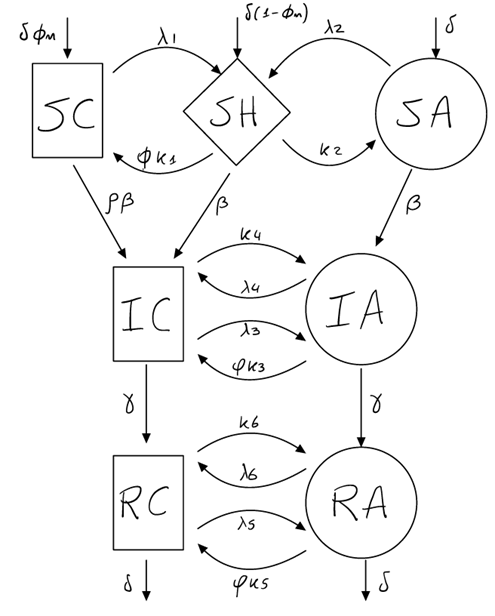
\includegraphics[width=0.5\linewidth]{1_corpo/figure/epi_behaviour_model_figure}
	\caption[Epidemic behavior model]{Figure of the epidemic behavior model with its compartment and influxes and out-fluxes.}
	\label{fig:epibehaviourmodelfigure}
\end{figure}

\subsection{Basic reproduction number calculation}
The first analysis that can be performed on the behavioral disease model is to estimate its basic reproduction number. It is defined as the spectral radius of the next-generation matrix. Using the method outlined in \cite{arino2007} and now briefly described this quantity is calculated. 
Consider a simple disease model in which $i \in R^n$ represents the set of infected compartments, $s \in R^n$ the set of susceptibles compartments, and $r \in R^k$ the set of compartments removed to the infection due to recovery. 

To describe the evolution of the system the following notation using matrices is adopted: 
\begin{itemize}
	\item $D$ is a $m \times m$ diagonal matrix; the diagonal elements are the relative susceptibilities of the corresponding susceptible class.
	\item $\Pi$ is a $n \times m$ matrix in which the $(k,j)$ element is the fraction of susceptible in the $j^{th}$ compartment that goes into the $k^{th}$ infective compartment.
	\item $b$ is an n-dimensional row vector of relative
	horizontal transmissions.
	\item $\beta'(s, i,r)$ multiplies the $b$ vector and is a scalar factor representing infectivity. It can be constant or a function of other parameters, such as incidence for example. 
	
	\item $V$ is a $n \times n$ matrix describing the transition between the infected state through death and recovery. 
	\item $g(s, i,r)$ is a continuous function representing the inlet of uninfected through birth or immigration. 
	\item $h(s, i, r)$ is also a function but used for the flow into and out of the recovered compartment because of natural immunity or vaccination.
\end{itemize} 

The resulting disease model is represented by the system:

\begin{equation}
	\begin{cases}
		s' = g(s,i,r) - D s \beta'(s,i,r) b i\\
		i' = \Pi D s \beta'(s,i,r) b i - V i\\
		r' = h(s,i,r) + W i \\		
	\end{cases}
	\label{eq:epi_ro_eq}
\end{equation}

Using the defined matrices, according to \cite{arino2007} the basic reproduction number $R_0$ for the model \eqref{eq:epi_ro_eq} at a disease free equilibrium $(s_0, 0, r_0)$ is given by:
\begin{equation}
R_0 = \beta'(s,i,r) b V^{-1} \Pi D s_0
\label{eq:R_0_eqn}
\end{equation}

The disease-free equilibrium is defined as a locally stable equilibrium of the system in which there is no disease and in the sense that a solution starting close to $(s_0, 0, r_0)$ remains close to this state. 

Considering the system dynamic presented in \eqref{eq:epi_behavioural_eq}, it can be rewritten in the matrix form expressed in  \eqref{eq:epi_ro_eq} as: 

\begin{align*}
\Pi & = 
\begin{bmatrix}
	\rho & 1 & 0 \\
	0 & 0 & 1
\end{bmatrix} &
D & = 
\begin{bmatrix}
	1 & 0 & 0 \\
	0 & 1 & 0\\
	0 & 0 & 1
\end{bmatrix} & 
s & = 
\begin{bmatrix}
	SC \\
	SH\\
	SA 
\end{bmatrix} \\
\\
b & = \begin{bmatrix}
	\epsilon & 1
\end{bmatrix} & 
V & = 
\begin{bmatrix}
	k_4 A + \lambda_3 + \gamma & - \phi k_3  C - \lambda_4\\
	- k_4 A - \lambda_3 & \phi k_3 C + \gamma + \lambda_4
\end{bmatrix} & 
i & = 
\begin{bmatrix}
	IC \\
	IA
\end{bmatrix}
\\
\end{align*}


The resulting $R_0$ find with this method is: 
\begin{figure}
	\centering
	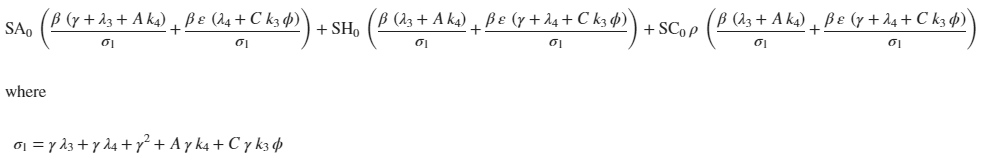
\includegraphics[width=0.99\linewidth]{1_corpo/figure/r0/ro_epidemic_behavioural}
	\caption[Reproduction number of epidemic behaviour model.]{Basic reproduction number of the epidemic behaviour model.}
	\label{fig:roepidemicbehavioural}
\end{figure}



\subsubsection{$I$ case: $R_0$ first evaluation}

A first evaluation of the $R_0$ is done using equation \eqref{eq:R_0_eqn} and assuming that at the beginning of an epidemic, the majority of the population is in the $SH$ compartment, while SC, SA, and also the A and C groups are close to zero. 
An initial tentative calculation for the value is done using a set of values assigned to the rest of the coefficients in the matrices.
For reference, the following values are used:

\begin{align*}
\beta &= 0.40  &\gamma &= 0.35 & \rho &= 0.65 &  \epsilon &= 0.15 \\
k_3 &= 0.49 & k_4 &= 0.243 & \lambda_3 &= 0.143 & \lambda_4 &= 0.143 \\
SC_0 & = 50/60e6 & SA_0 &= 50/60e6 & C &= A = SC_0 & SH_0 & = 1 - SC_0- SA_0\\ 	
\end{align*}


With these coefficient values, considering separately the epidemic and behavioral layers the basic reproduction values are:
 \begin{align*}
 	R_0^{SIR} &= \frac{\beta}{\gamma} = 1.1429 \\
 	R_3^{behav} & = \frac{k_3}{\lambda_3} =  3.3566  \\
 	R_4^{behav} & = \frac{k_4}{\lambda_4} = 1.6993 \\
 \end{align*}
   
In this situation, an epidemic can spread, in fact $R_0^{SIR} >1$, and looking at the behavior of people the complaints, associated with $R_3^{behav}$, have a larger influence than the one of the "against" group.

The epidemic-behaviour reproduction number found using the formula and assuming an initial awareness equal to $0.5$ is 
\[R_0^{epi-behav} = 0.3898\]

It is immediately noticed that the reproduction number is way below the threshold value of 1. According to the theorem presented in \cite{arino2007} there cannot be the spread of disease if the initial $R_0$ is under this value. A simulation of the system dynamic confirms this situation. Observing figure \ref{fig:infected00_epi_behav} can be seen that the number of infected tends to decrease and goes to zero. Then the majority of the population remains in the Susceptible compartment, splitting into compliant and heedless subgroups. This is due to the strongest attractivity of compliant behavior simulated in this scenario.  

\begin{figure}[ht]
	\centering
	\subfloat[][\emph{Susceptibles compartments}]
	{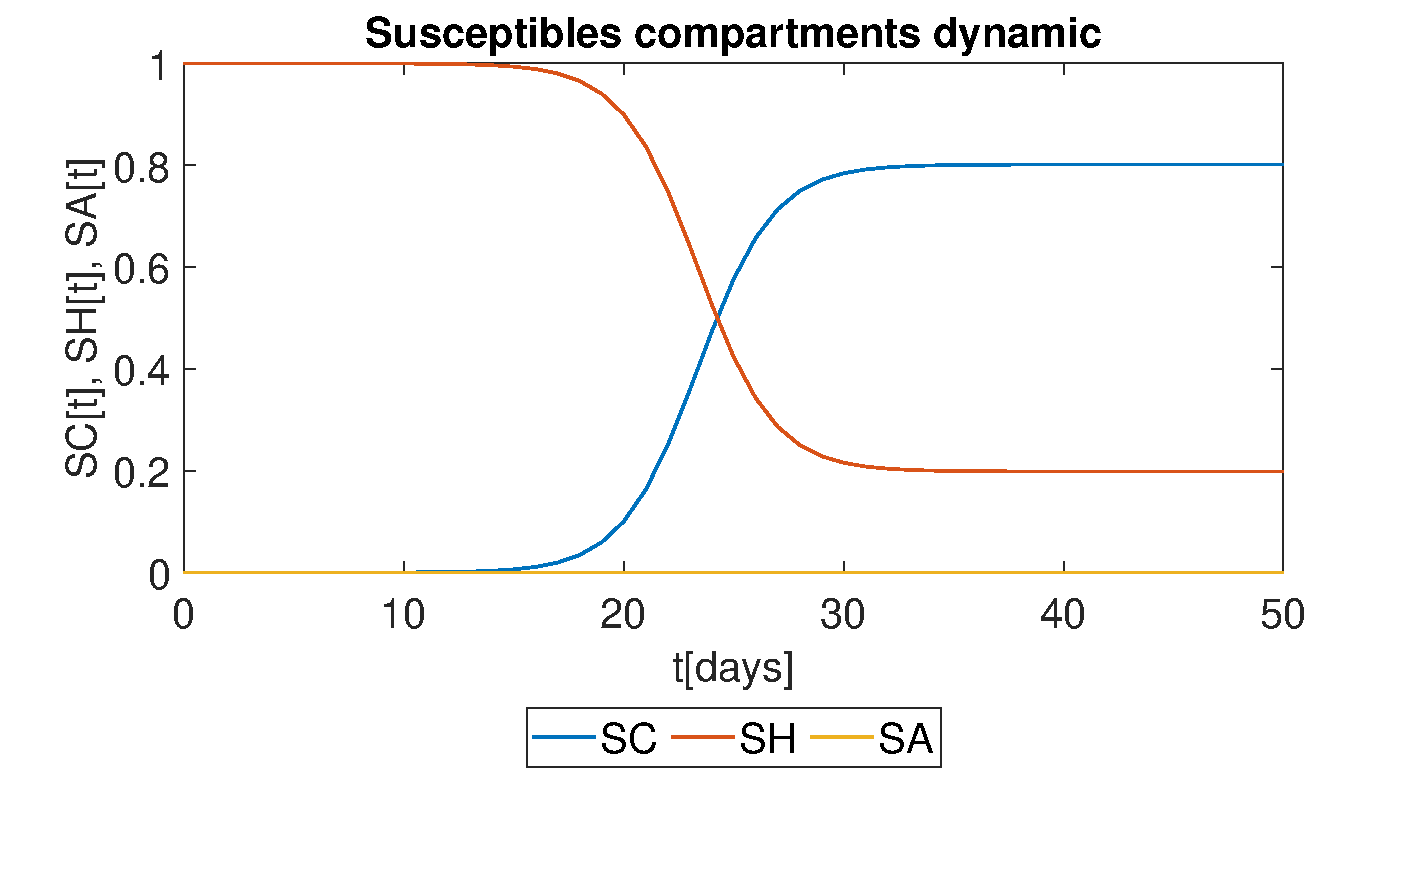
\includegraphics[width=.45\textwidth]{1_corpo/figure/r0/susceptible00_epi_behav}} \quad
	\subfloat[][\emph{Infected compartments}]
	{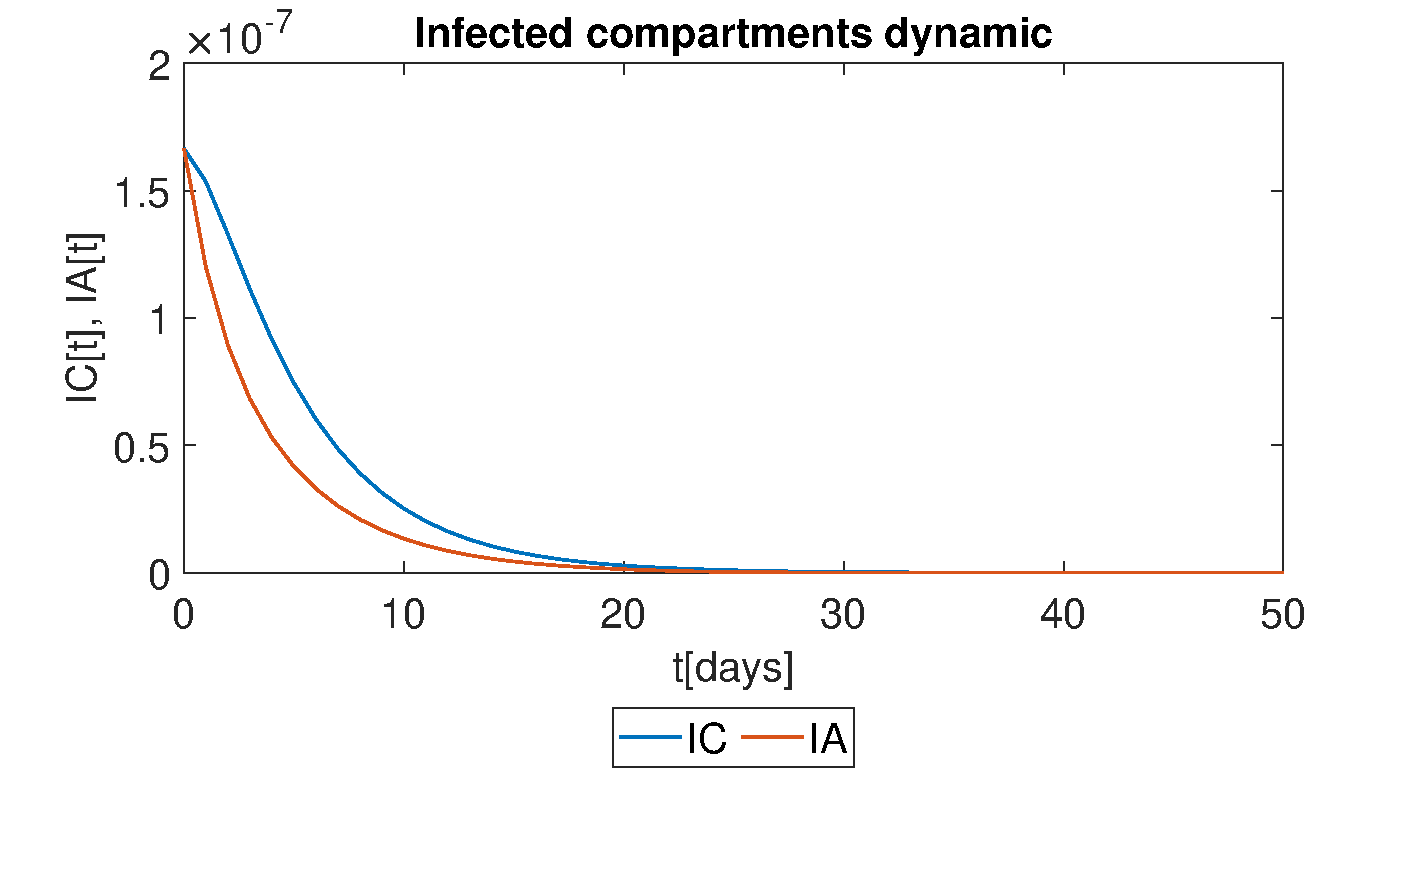
\includegraphics[width=.45\textwidth]{1_corpo/figure/r0/infected00_epi_behav}} \\
	\subfloat[][\emph{Recovered compartment}]
	{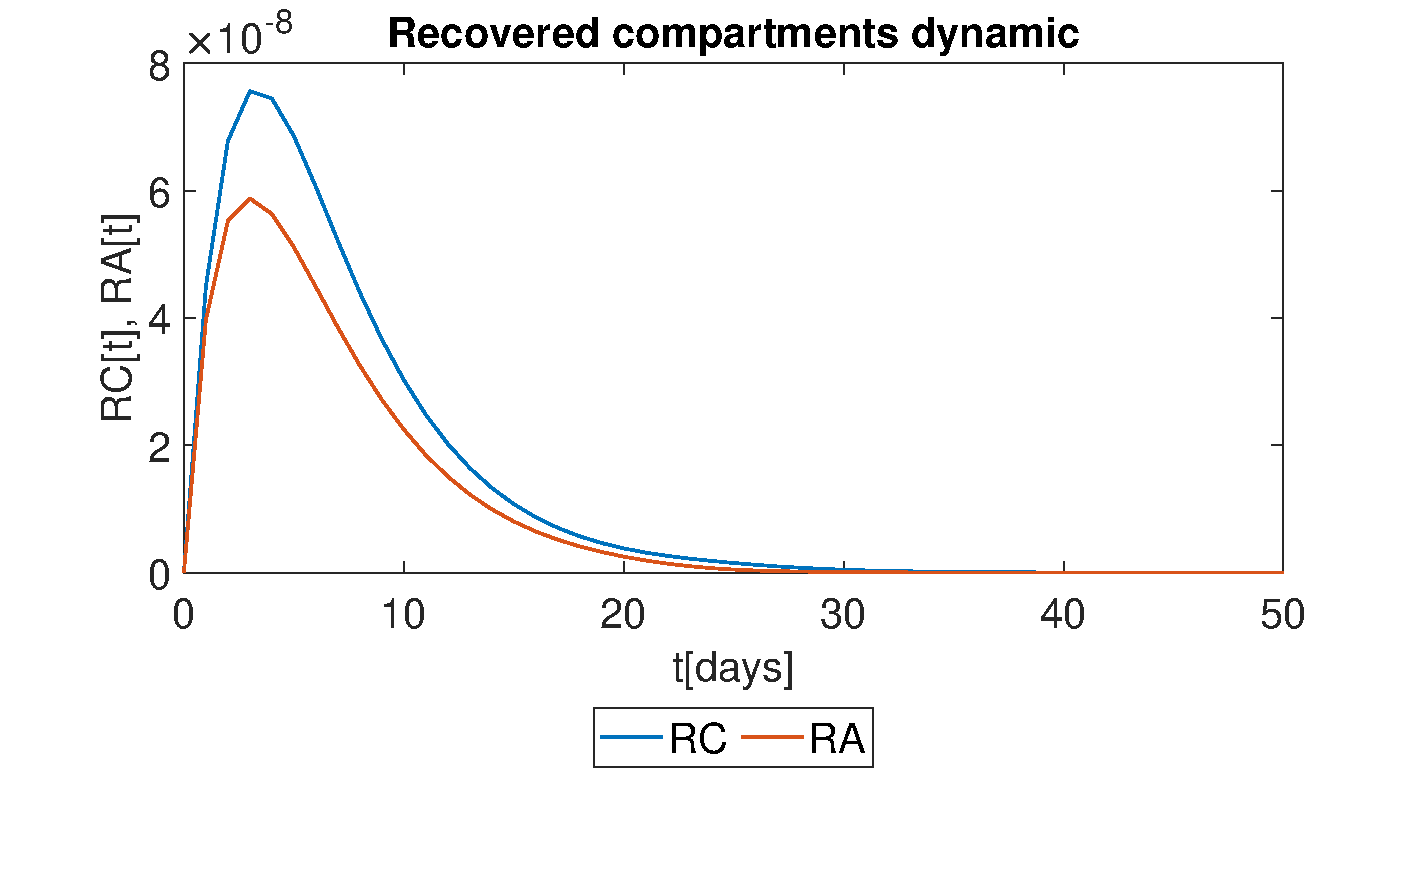
\includegraphics[width=.45\textwidth]{1_corpo/figure/r0/recovered00_epi_behav}}
	\caption[Epidemic behavioral model $R_0$]{Evolution of the behavioral epidemic model, with fixed parameters for the coefficients and an initial reproduction rate less than $1$. It is observed that there aren't conditions for an epidemic to spread.}
	\label{fig:infected00_epi_behav}
\end{figure}

\subsubsection{$II$ case: how parameters influence the $R_0$ value}

A second test performed on the find $R_0^{epi-behav}$ wants to understand what are the parameters that influence more its value. The aim is to find which combination of coefficients can have a critical impact in the first phase of the disease and cause an overshoot of the threshold value. The value of the reproductive rate is then calculated varying the coefficients and the results are now presented in \ref{fig:r0_epi_behav_coef}. 

\begin{figure}[ht]
	\centering
	\subfloat[][\emph{$R_0$ varying the initial population value in susceptible compliant and susceptible against group. The more the population is against the higher the reproductive ratio.}]
	{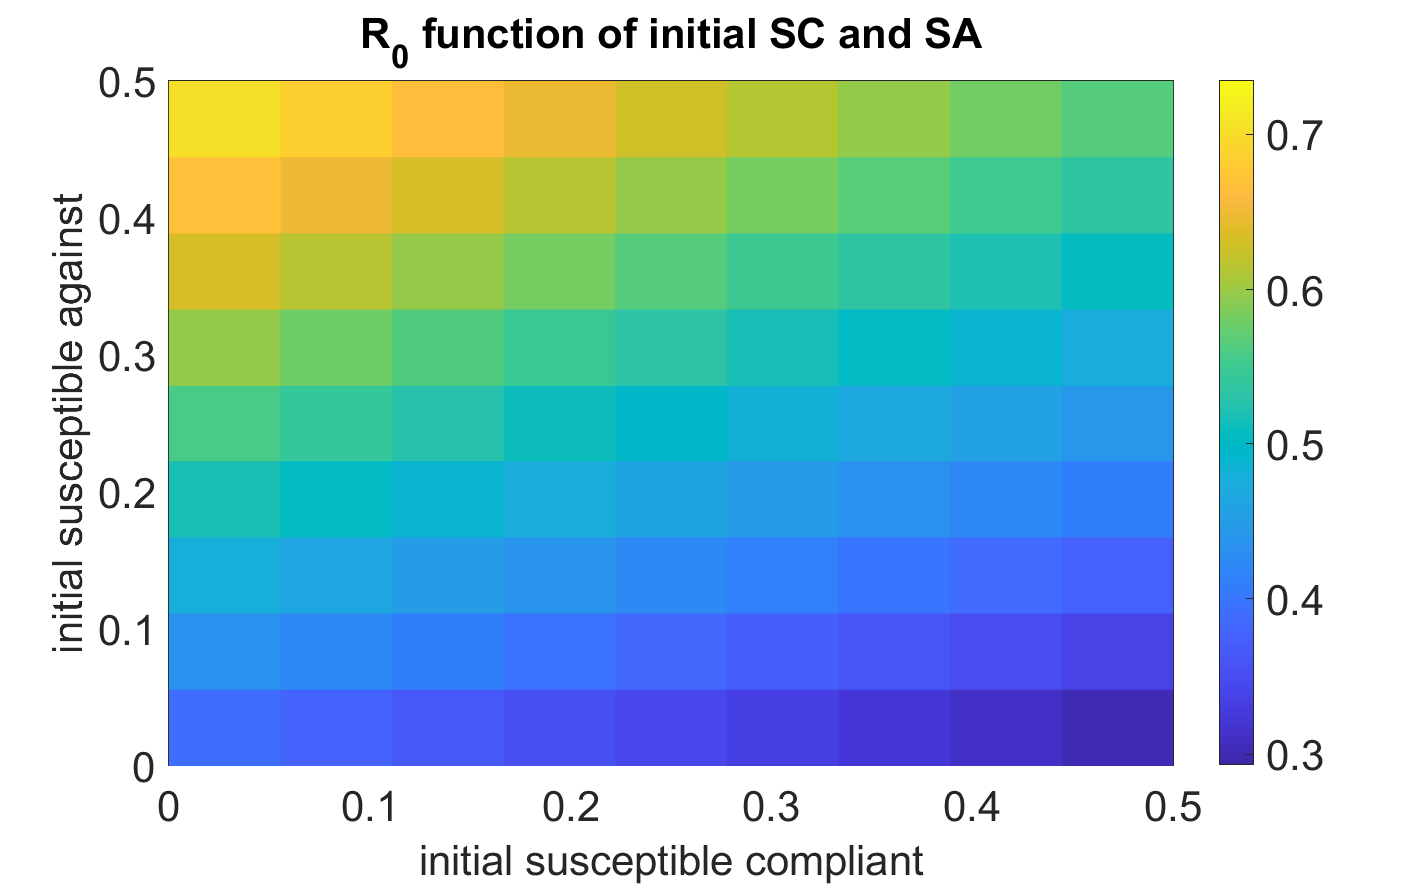
\includegraphics[width=.45\textwidth]{1_corpo/figure/r0/r0_epi_behav_SC_SA}} \quad
	\subfloat[][\emph{$R_0$ varying the number of initial compliant susceptible and the parameter ruling the efficacy of adopting a safe behavior and avoiding contracting the disease. The lower is $\rho$ the higher is the probability of not becoming infected.}]
	{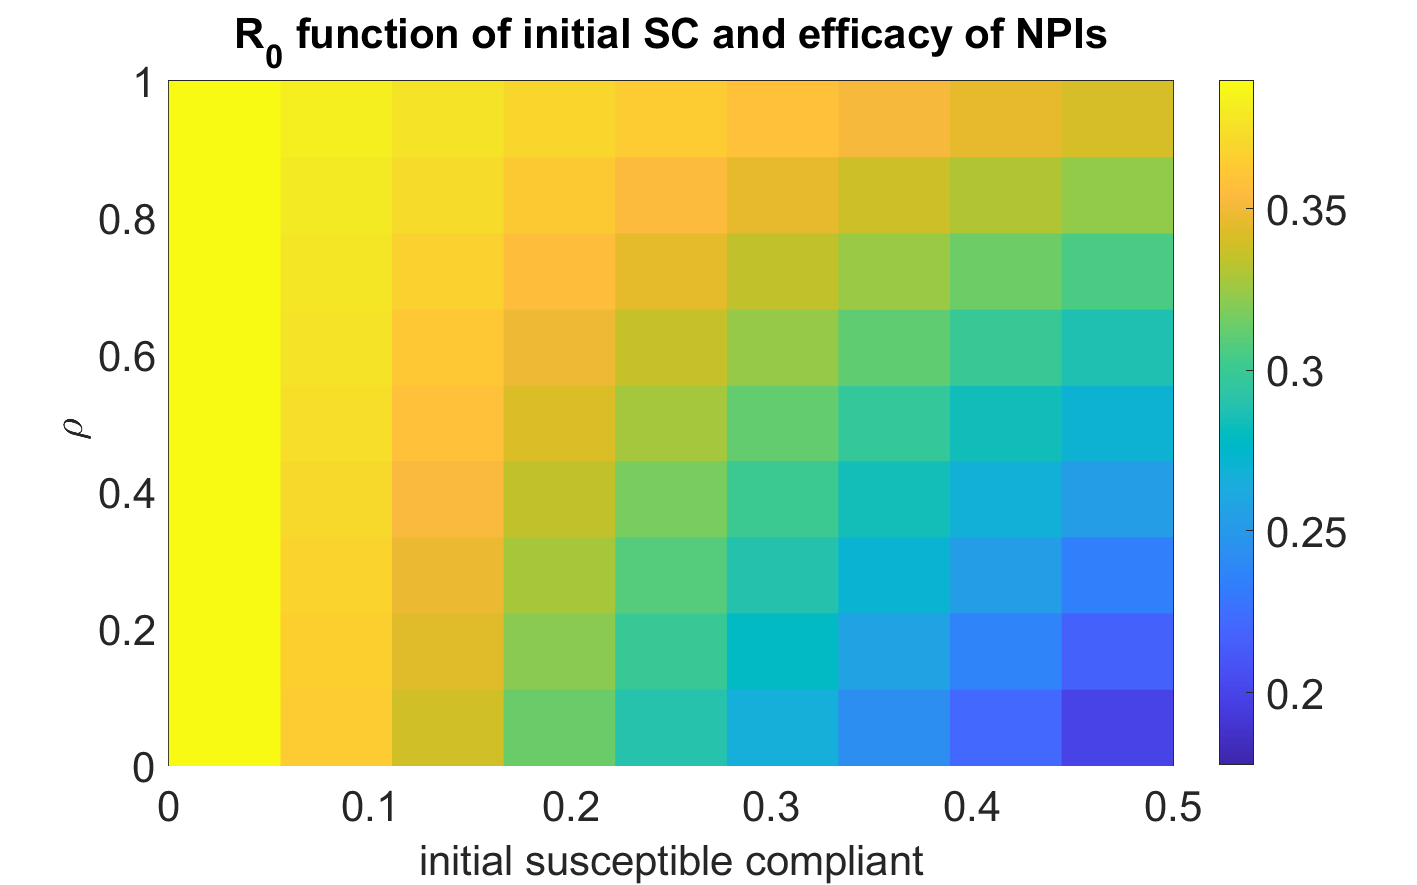
\includegraphics[width=.45\textwidth]{1_corpo/figure/r0/r0_epi_behav_SC_rho}} \\
	\subfloat[][\emph{The influence of the awareness parameter on the $R_0$.}]
	{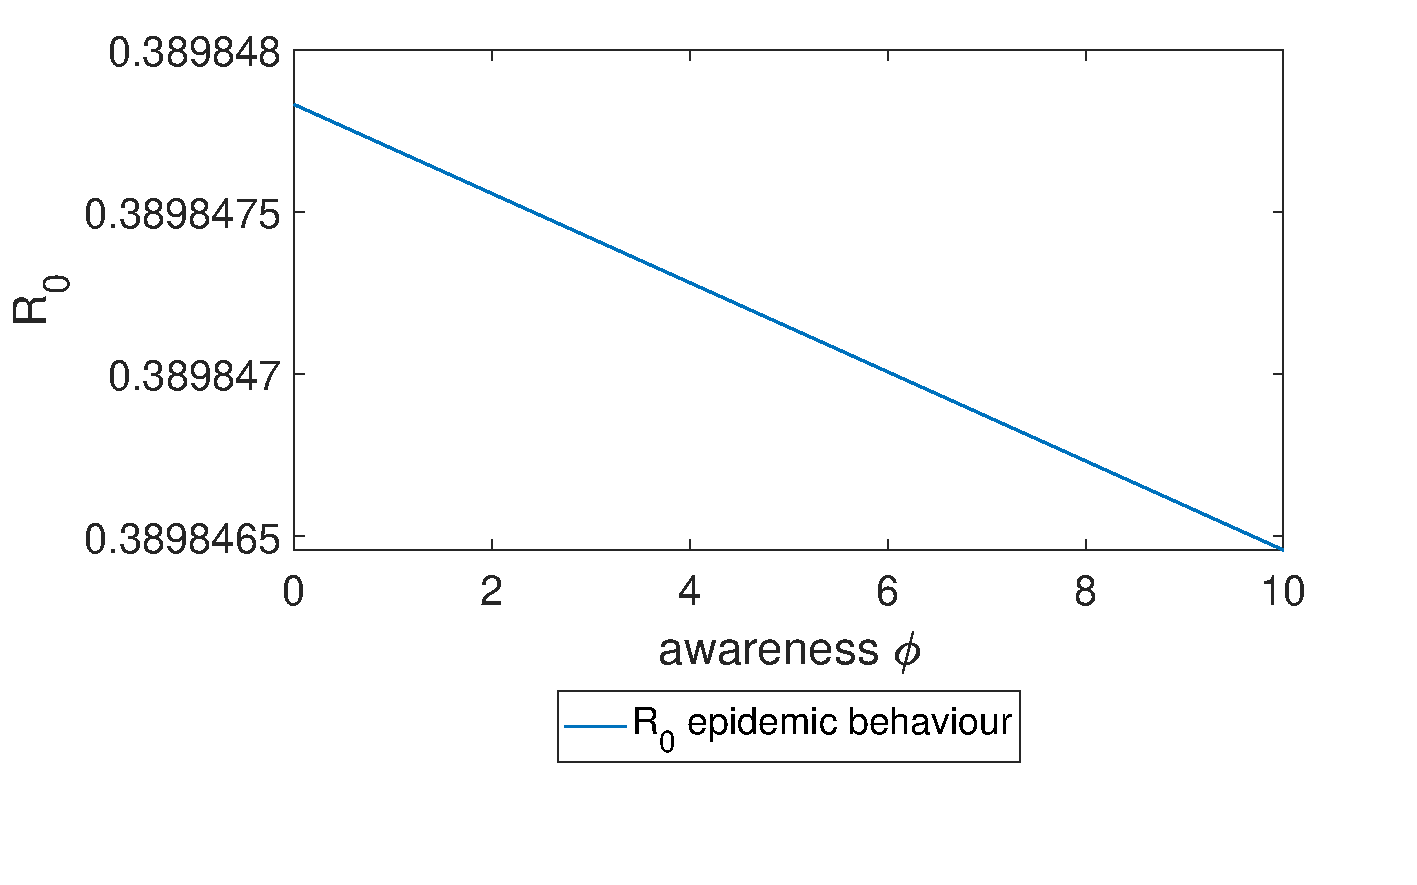
\includegraphics[width=.45\textwidth]{1_corpo/figure/r0/r0_epi_behav}}
	\caption[Epidemic behavioral $R_0$ coefficients ]{Value of $R_0^{epi-behav}$ varying some parameters and maintaining constant all the other initial conditions.}
	\label{fig:r0_epi_behav_coef}
\end{figure}


The case shown in figure \ref{fig:r0_epi_behav_coef} is an example of how changes the reproductive rate value. The most interesting observation is that the value of awareness practically does not modify the $R_0^{epi-behav}$. Instead, it can be observed a threshold in the number of initial susceptible compliant for which the reproductive rate becomes smaller, depending on the efficacy of the protective behavior. If there are less than $5\%$ of the population in the compliant group, for any value of $\rho$ the reproductive rate does not change. 